\chapter{幂函数、指数函数与对数函数}
上一章,通过“函数概论”的学习初步理解了研究函数的
基本途径和方法。本章将运用这些思想研究几类重要的初等
函数:幂函数、指数函数和对数函数。

\section{幂函数}
我们已经学过函数$y=x$, 
$y=x^2$
和
$y=x^{-1}$(即
$y=\frac{1}{x}$),
这些都是幂函数。

一般地,函数$y=x^{\alpha}$
($\alpha$是常数,
$\alpha\in\R$)
叫做幂函数,其
中$x$是自变量。

限于知识水平,本章只研究$\alpha$为有理数的情况,此时记
作
$y=x\; (n\in \Q)$.

先讨论幂函数
的定义域。

\begin{enumerate}[(1)]
    \item $n$为正整数时,$x^n$
的意义是$x=x\cdot x\cdots$(共有
$n$个$x$相乘)其定义域为
$D=(-\infty,+\infty)$;
\item $n$为正分数时,我们只研究$n$是既约分数$\frac{p}{q}$
的情况($p$、$q$是正整数,且
$q\ge 2$)这时$x^n$
的意义是$x^{\tfrac{p}{q}}=\sqrt[q]{x^p}$,函数定义域为使$\sqrt[q]{x^p}$有意义的实数$x$的集合,即当$q$
为奇数时,定义域
$D=(-\infty,+\infty)$,$q$
为偶数时($p$必为奇数),定
义域
$D=[0,+\infty)$
\item $n=0$时,$x^n=x^0$
,定义域
$D=(-\infty,0)\cup (0,+\infty)$;
\item $n$是负整数时,设
$n=-m,\; x^n=x^{-m}=\frac{1}{x^m},\; (m\in\N)$,
其定义域为$D=(-\infty,0)\cup (0,+\infty)$;
\item $n$是负分数时,
$n=-\frac{p}{q}$($p,q$为互质的正整数,
且$q\ge 2$)时,
\[x^n=\frac{1}{x^{\tfrac{p}{q}}}=\frac{1}{\sqrt[q]{x^p}}\]
当$q$为奇数时,定义域为
$D=(-\infty,0)\cup (0,+\infty)$; $q$为偶数时,
$D=(0,+\infty)$.

\end{enumerate}

总之,对于幂函数
$y=x^n\; (n\in\Q)$
来说,\textbf{使$x^n$
有意义的实
数$x$的集合就是它的定义域}。

\begin{example}
    说出下列幂函数的定义域:
\[y=x^0,\quad y=x^3,\quad y=x^{-2},\quad y=x^{\tfrac{1}{3}},\quad y=x^{\tfrac{1}{2}},\quad y=x^{-\tfrac{1}{2}}\]
\end{example}

\begin{solution}
$y=x^{0}$和$y=x^{-2}$的定义域为$(-\infty,0)\cup (0,+\infty)$;

$y=x^3$ 和 $y=x^{\tfrac13}$的定义域都是$(-\infty; +\infty)$;

$y=x^{\tfrac12}$的定义域为$[0, +\infty)$,\quad  $y=x^{-\tfrac12}$的定义域为$(0,+\infty)$。

\end{solution}

以下研究幂函数的图象和性质。

当$n=0$ 时,$y=x^{n}=1\; (x\neq0)$, 它的图象是与$y=1$ 重合
的一条直线 (除去点$(0,1)$).

下面着重研究$n\neq0$的情况。

当$n$是整数时。若$n$是奇数,可知$y=x^{n}$为奇函数,其图
象关于坐标原点对称,且图象在第一、三象限内;若$n$是偶
数,可知$y=x^n$
为偶函数,其图象关于$y$轴对称,且图象在第
一、二象限内;

当$n$为既约分数$\frac pq$($p$、$q$为整数,$q{\geq}2$, $p{\neq}0$)时:若 $q$、$p$ 均为奇数,可知函数$y=x^{\tfrac pq}$为奇函数,图象关 于 坐标原点对称,且图象在第一、三象限内;若$q$为奇数,$p$为偶数,可知函 数 $y=x^{\tfrac pq}$为偶函数,图象关于$y$轴对称,且图象在第一、二象限内;若$q$为偶数($p$ 只能是奇数), 可知函数$y=x^{\tfrac pq}$为非奇非偶函数,且图象只在第一象限内。

综上所述,只要把函数$y=x^n$ 在第一象限内的图象及其
特征搞清了,问题便迎刃而解。

\subsection{$n>0$时}
在同一坐标系内画出
$y=x^3$, $y=x^2$, $y=x$, $y=x^{\tfrac{1}{2}}$,$y=x^{\tfrac{1}{3}}$
在区间$[0,+\infty)$
上的图象如下:
\begin{figure}[htp]
    \centering
\begin{tikzpicture}[>=stealth, scale=2]
\draw[->](-.5,0)--(3,0)node[right]{$x$};
\draw[->](0,-.5)--(0,3)node[right]{$y$};
\draw[domain=0:2.5, smooth, very thick]plot(\x, \x)node[right]{$y=x$};
\draw[domain=0:1.5, smooth, very thick]plot(\x, \x^2)node[right]{$y=x^2$};
\draw[domain=0:1.35, smooth, very thick]plot(\x, \x^3)node[above right]{$y=x^3$};
\draw[domain=0:1.5, smooth, very thick]plot(\x^2,\x)node[above right]{$y=x^{\tfrac{1}{2}}$};
\draw[domain=0:1.35, smooth, very thick]plot(\x^3,\x)node[right]{$y=x^{\tfrac{1}{3}}$};
\draw[dashed](0,1)node[left]{1}--(1,1)--(1,0)node[below]{1};
\node[below left]{$O$};


\end{tikzpicture}
    \caption{}
\end{figure}

由图3.1可见,幂函数$y=x^n\; (n>0)$,当$x\in[0,+\infty)$时:
\begin{enumerate}[(1)]
\item 图象都过点$(0,0)$和$ (1, 1)$,
\item 都是单调增函数,
\item 对于$n_1>n_2>0$, 若$x_0\in ( 1, + \infty) $时,有$x_0^{n_1}>x_0^{n_2}$; 若$x_0\in(0,1)$ 时,$x_0^{n_1}<x_0^{n_2}$.
\end{enumerate}

\begin{example}
    讨论函数$y=x^{\tfrac{2}{3}}$
的定义域、值域、奇偶性,画出它的图象,并说明函数的单调区间。
\end{example}

\begin{solution}
函数$y=x^{\tfrac{2}{3}}=\sqrt[3]{x^2}$
,定义域为$(-\infty,+\infty)$,值域
为$[0,+\infty)$,由于
$f(-x)=\sqrt[3]{(-x)^2}=\sqrt[3]{x^2}=f(x)$
,所以
函数为偶函数。

图象关于$y$
轴对称。图象过$(0,0)$, $(1,1)$,
$(-1,1)$点:

由图3.2可知,幂函数
$y=x^{\tfrac{2}{3}}$
的单调增区间为$(0,+\infty)$
,单调减区间为$(-\infty,0)$.
\end{solution}





\begin{figure}[htp]
    \centering
\begin{minipage}{.6\textwidth}
\begin{tikzpicture}[>=stealth, scale=.6]
    \draw[->](-6,0)--(6,0)node[right]{$x$};
    \draw[->](0,-.5)--(0,5)node[right]{$y$};
    \draw[domain=0:5.75, smooth, very thick]plot(\x, {\x^(2/3)})node[above]{$y=x^{\tfrac{2}{3}}$};
    \draw[domain=0:5.75, smooth, very thick]plot(-\x, {\x^(2/3)});
\foreach \x in {-5,-3,-1,1,3,5}
{
    \draw(\x,0)node[below]{$\x$}--(\x,.2);
}
\draw[dashed](-1,1)--(1,1);
\node at (0,4)[right]{4};
\node at (0,2)[right]{2};
\draw[dashed](-2.828,2)--(2.828,2);
\draw[dashed](-1.732*3,3)--(1.732*3,3);
\draw(0,4)--(-.2,4);

\node[below right]{$O$};

\end{tikzpicture}
    \caption{}
\end{minipage}    \hfill
\begin{minipage}{.3\textwidth}
\begin{tikzpicture}[>=stealth]
    \draw[->](-.5,0)--(3,0)node[right]{$x$};
    \draw[->](0,-.5)--(0,3)node[right]{$y$};
    \draw[domain=0:2.5, smooth, very thick]plot(\x, {\x^(3/4)})node[above]{$y=x^{\tfrac{3}{4}}$};
\foreach \x in {1,2}
{
    \draw(\x,0)node[below]{\x}--(\x,.1);
    \draw(0,\x)node[left]{\x}--(.1,\x);
}
\node[below left]{$O$};

\end{tikzpicture}
\caption{}
\end{minipage}
\end{figure}






\begin{example}
画出函数$y=x^{\tfrac{3}{4}}$
的图象(草图),并说明其增减性。    
\end{example}

\begin{solution}
    应先讨论函数的性质,再画图象。

函数$y=x^{\tfrac{3}{4}}$的定义域为$[0,+\infty)$,
值域为$[0,+\infty)$,
为非奇非偶函数,图象在第一象限(含原点),见图3.3.

由图象可知,函数$y=x^{\tfrac{3}{4}}$
为单调增函数。
\end{solution}

\subsection{$n<0$时}
在同一坐标系内,画出
$y=x^{-2}$,$y=x^{-1}$和
$y=x^{-\tfrac{1}{2}}$
在区间$(0,+\infty)$
上的图象:

\begin{figure}[htp]
    \centering
\begin{tikzpicture}[>=stealth, scale=2]
    \draw[->](-.5,0)--(3.5,0)node[right]{$x$};
    \draw[->](0,-.5)--(0,3.5)node[right]{$y$};
    \draw[domain=0.55:2.5, smooth, very thick]plot(\x, {\x^(-2)})node[right]{$y=x^{-2}$};
    \draw[domain=0.3:2.5, smooth, very thick]plot(\x, {\x^(-1)})node[right]{$y=x^{-1}$};    
    \draw[domain=0.1:2.5, smooth, very thick]plot(\x, {\x^(-0.5)})node[above right]{$y=x^{-\tfrac{1}{2}}$};
\foreach \x in {1,2,3}
{
    \draw(\x,0)node[below]{\x}--(\x,.1);
    \draw(0,\x)node[left]{\x}--(.1,\x);
}
\node [below left]{$O$};
\draw[dashed](0,1)--(1,1)node[above right]{$(1,1)$}--(1,0);


\end{tikzpicture}
    \caption{}
\end{figure}

由图3.4可见,幂函数$y=x^n\; (n<0)$,当$x\in(0,+\infty)$时:
\begin{enumerate}[(1)]
    \item 图象都过点$(1,1)$;
    \item 都是单调减函数;
    \item 在第一象限内,图象向上与$y$轴无限地接近,向
    右与$x$轴无限地接近。称图象分别以$y$
    轴和$x$轴为\textbf{渐近线}。
    \item 对于$n_1<n_2<0$时, 若$x_0\in(1,+\infty)$时, 有$x_0^{n_1}<x_0^{n_2}$; 若$x_0\in(0,1)$时, $x_0^{n_1}>x_0^{n_2}$.
\end{enumerate}

\begin{example}
    在同一坐标系内,画出函数 $y= x^{-\tfrac{1}{2}}$, $ y= x^{\tfrac{1}{3}}$ 和
$y=x^{-2}$的图象。
\end{example}

\begin{solution}
    首先根据上述 $y=x^n$ 的图象和性质,作出这三个函
数在第一象限内的图象,再根据它们各自的奇偶性,分别作
出它们各自的完整的图象(图3.5)。
\end{solution}

\begin{figure}[htp]
    \centering
\begin{tikzpicture}[>=stealth, scale=1.5]
    \draw[->](-2.5,0)--(3,0)node[right]{$x$};
    \draw[->](0,-1.5)--(0,2.5)node[right]{$y$};
    \draw[domain=0.25:2.5, smooth, very thick]plot(\x, {\x^(-1/2)})node[above right]{$y=x^{-\tfrac12}$};
    \draw[domain=0:2.5, smooth, samples=100]plot(\x, {\x^(1/3)})node[above right]{$y=x^{\tfrac13}$};    
    \draw[domain=0.65:2.5, smooth, ultra thick]plot(\x, {\x^(-2)})node[right]{$y=x^{-2}$};
\foreach \x in {1,2}
{
    \draw(\x,0)node[below]{\x}--(\x,.1);
    \draw(0,\x)node[left]{\x}--(.1,\x);
}
\node [below left]{$O$};
\draw[dashed](0,-1)node[right]{$-1$}--(-1,-1)--(-1,0)node[below left]{$-1$}--(-1,1)--(1,1)--(1,0);

\draw[domain=0.65:2.5, smooth, ultra thick]plot(-\x, {\x^(-2)})node[above right]{$y=x^{-2}$};

\draw[domain=0:2.5, smooth, samples=100]plot(-\x, -{\x^(1/3)})node[below right]{$y=x^{\tfrac13}$};   

\end{tikzpicture}
    \caption{}
\end{figure}

\begin{note}
    本例题给出了作幂函数图象的步骤。
\begin{enumerate}[(1)]
    \item 先作出第一象限内的图象,
\item 若幂函数的定义域为$(0, +\infty)$(或$[0,+\infty)$),
作图已完成;若在$(-\infty,0)$或$(-\infty,0]$上有意义,则
只需根据函数的奇偶性,利用其图象的对称关系,作出第一象限图象关于原点或$y$轴的对称图象即可。
\end{enumerate}
\end{note}


\begin{example}
    比较下列各组数的大小:
 \begin{multicols}{2}
 \begin{enumerate}[(1)]
     \item $1.5^{\tfrac{2}{3}}$与$1.7^{\tfrac{2}{3}}$
     \item $\left(\sqrt{3}\right)^{\tfrac{5}{4}}$与$\left(\frac{5}{3}\right)^{\tfrac{5}{4}}$
     \item $3.14^{-\tfrac{4}{3}}$与$\pi^{-\tfrac{4}{3}}$
     \item $(-6.3)^{\tfrac{4}{3}}$与$(-6.4)^{\tfrac{4}{3}}$
     \item $\left(-\sqrt{2}\right)^{-\tfrac{3}{5}}$与$\left(-\sqrt{3}\right)^{-\tfrac{3}{5}}$
 \end{enumerate}
 \end{multicols}
 \end{example}
 
 \begin{analyze}
     各题中的两个值都是“同指数”的幂,因此可看作是同一个幂函数的两个不同的函数值。从而可据幂函数的单调性做出判断.
 \end{analyze}
 
 \begin{solution}
 \begin{enumerate}[(1)]
     \item 由于幂函数$y=x^{\tfrac{2}{3}}\; (x>0)$单调递增,且$1.5<1.7$
 
     $\therefore\quad 1.5^{\tfrac{2}{3}} < 1.7^{\tfrac{2}{3}}$
 \item 由于幂函数$y=x^{\tfrac{5}{4}}\; (x>0)$单调递增,且$\sqrt{3}>\frac{5}{3}$
 
 $\therefore\quad \left(\sqrt{3}\right)^{\tfrac{5}{4}} > \left(\frac{5}{3}\right)^{\tfrac{5}{4}}$
 \item 由于幂函数$y=x^{-\tfrac{4}{3}}\; (x>0)$单调递减,且$3.14<\pi$
 
 $\therefore\quad 3.14^{-\tfrac{4}{3}} < \pi^{-\tfrac{4}{3}}$
 \item 由于幂函数$y=x^{\tfrac{4}{3}}$是偶函数
 
 $\therefore\quad f(-x)=f(x)$,由此:
 \[(-6.3)^{\tfrac{4}{3}}=6.3^{\tfrac{4}{3}},\qquad (-6.4)^{\tfrac{4}{3}}=6.4^{\tfrac{4}{3}}\]
 而$y=x^{\tfrac{4}{3}}\; (x>0)$单调递增,且$6.3<6.4$,
 
 $\therefore\quad 6.3^{\tfrac{4}{3}} < 6.4^{\tfrac{4}{3}}$,从而:$(-6.3)^{\tfrac{4}{3}} < (-6.4)^{\tfrac{4}{3}}$
 \item 由于幂函数$y=x^{-\tfrac{3}{5}}$是个奇函数
 
 $\therefore\quad f(-x)=-f(x)$,由此
 \[\left(-\sqrt{2}\right)^{-\tfrac{3}{5}}=-\left(\sqrt{2}\right)^{-\tfrac{3}{5}},\qquad \left(-\sqrt{3}\right)^{-\tfrac{3}{5}}=-\left(\sqrt{3}\right)^{-\tfrac{3}{5}}\]
 
 而$y=x^{-\tfrac{3}{5}}\; (x>0)$单调递减,且$\sqrt{2}<\sqrt{3}$
 
 $\therefore\quad \left(\sqrt{2}\right)^{-\tfrac{3}{5}}>\left(\sqrt{3}\right)^{-\tfrac{3}{5}}\Longrightarrow -\left(\sqrt{2}\right)^{-\tfrac{3}{5}}<-\left(\sqrt{3}\right)^{-\tfrac{3}{5}}$
 
 $\therefore\quad \left(-\sqrt{2}\right)^{-\tfrac{3}{5}}< \left(-\sqrt{3}\right)^{-\tfrac{3}{5}}$
 \end{enumerate}
 \end{solution}
 
 \begin{note}
 (4)、(5)两题中,我们是利用幂函数的奇、偶
     性,先把底为负数的幂转化为正数的幂解决问题。当然,若直接利用$x<0$上的幂函数的单调性解决问题也是可行的。
 \end{note}
 
 \begin{example}
 求函数$y=(x-3)^{-2}$的定义域,并讨论其增减性。  
 \end{example}
 
 \begin{solution}
 \[y=(x-3)^{-2}=\frac{1}{(x-3)^2}\]
 定义域为$D=(-\infty,3)\cup (3,+\infty)$.
 
 因为$y=(x-3)^{-2}$可看作是由函数$y=x^{-2}$的图象向右平移3个单位后的结果,所以,当$x\in (-\infty,3)$时,函数单调递增;而当$x\in(3,+\infty)$时,函数单调递减。
 \end{solution}
 
 \begin{note}
     把所要研究的问题\underline{化归}为熟知的事实,这是数学中处理问题的常用思维方式。
 \end{note}
 
 
 \section*{习题一}
 \begin{center}
     \bfseries A
 \end{center}
 
 \begin{enumerate}
     \item 写出下列函数的定义域,值域,并讨论其奇偶性:
 \begin{multicols}{2}
 \begin{enumerate}[(1)]
     \item $y=x^{-2}$
     \item $y=x^{\tfrac{5}{7}}$
     \item $y=x^{\tfrac{4}{5}}$
     \item $y=x^{\tfrac{5}{6}}$
     \item $y=x^{-\tfrac{3}{2}}$
     \item $y=x^{-\tfrac{4}{5}}$
 \end{enumerate}
 \end{multicols}
     \item 写出下列函数的定义域,并讨论其奇偶性:
 \begin{multicols}{2}
 \begin{enumerate}[(1)]
     \item $f_1(x)=x^2+x^{-2}$
     \item $f_2(x)=x+3x^{\tfrac{2}{3}}$
     \item $f_3(x)=2x+\sqrt[3]{x}$
     \item $f_4(x)=2x^{-4}-3x^{-2}$
 \end{enumerate}    
 \end{multicols}
 \item 讨论下列函数的定义域、值域、奇偶性,并画出函数的图象:
 \begin{multicols}{3}
 \begin{enumerate}[(1)]
     \item $y=x^{\tfrac{3}{4}}$
     \item $y=x^{-\tfrac{2}{3}}$
     \item $y=x^{-\tfrac{1}{2}}$
 \end{enumerate}
 \end{multicols}
 
 \item 在同一坐标系内,画出下列各题中的两个函数的图象,并加以比较:
 \begin{multicols}{2}
 \begin{enumerate}[(1)]
     \item $y=x^3,\quad y=x^4$
     \item $y=x^{-3},\quad y=x^{-4}$
 \end{enumerate}
 \end{multicols}
 
 \item 比较下列各题中两个值的大小:
 \begin{multicols}{2}
 \begin{enumerate}[(1)]
     \item $2.3^{\tfrac{3}{4}}$与$2.4^{\tfrac{3}{4}}$
     \item $0.7^{\tfrac{2}{3}}$与$0.8^{\tfrac{2}{3}}$
     \item $\left(\sqrt{2}\right)^{-\tfrac{3}{2}}$与$\left(\sqrt{3}\right)^{-\tfrac{3}{2}}$
     \item $1.1^{-\tfrac{1}{2}}$与$0.9^{-\tfrac{1}{2}}$
     \item $\left(\frac{3}{7}\right)^{-\tfrac{4}{3}}$与$\left(\frac{5}{8}\right)^{-\tfrac{4}{3}}$
     \item $(-\pi)^{\tfrac{2}{3}}$与$(-3.1)^{\tfrac{2}{3}}$
     \item $\left(-\frac{10}{11}\right)^{\tfrac{3}{5}}$与$\left(-\frac{11}{12}\right)^{\tfrac{3}{5}}$
 \end{enumerate}
 \end{multicols}
 
 \end{enumerate}
 
 \begin{center}
     \bfseries B
 \end{center}
 
 \begin{enumerate}\setcounter{enumi}{5}
     \item 求函数$y=(x+2)^{-2}$的定义域、值域,画出它的图象,并写出它的单调区间。
 \item     把幂函数$y=x^r\; (r\in\Q)$的图象经过怎样平移,可得到$y=(x+m)^r+n\; (mn\ne 0)$的图象?
 \item     把幂函数$y=\frac{1}{x}$的图象经过怎样平移,可得到
     $y=\frac{3x+7}{x+2}$的图象?
 \end{enumerate}
 
 
 \begin{center}
     \bfseries C
 \end{center}
 
 \begin{enumerate}\setcounter{enumi}{8}
 \item \begin{enumerate}[(1)]
     \item 由$y=x$的图象,经过取倒数变换画出$y=\frac{1}{x}$的图象(草图)。
     \item 由$y=x^3$的图象,经过取倒数变换画出$y=x^{-3}$的图象(草图)。
     \item 由$y=x^{\tfrac{1}{2}}$的图象,经过取倒数变换可以画出哪个函数的图象?试画一下。
 \end{enumerate}
 \end{enumerate}
 
 \section{指数函数}
 \subsection{指数函数的概念}
     
 在幂函数$y=x^{\alpha}$(常数$\alpha\in\R$)中,底数是自变量,指数$\alpha$是常数,即“底数变、指数不变”。若令“底数不变、指数变”,如$y=2^x,\; y=10^x\; y=\left(\frac{1}{2}\right)^x$等等,则称$y$是$x$的指数函数。
 
 一般地,函数$y=a^x$ $(0<a\ne 1)$叫\textbf{指数函数},自变量为$x$。其中$a$是不等于1的正常数\footnote{当$a>0$时,若$x$是无理数,$a^x$是一个确定的实数;对于无理指数幂,过去学过的有理指数幂的性质和运算法则都适用,有关概念与定理证明在本书中从略.
 
 若$a=1$, $y=1^x$极其简单,没有研究的价值.
 
 若$a<0$, $y=a^x$不是对任意实数$x$都有意义,并且极为复杂,因此我们也不去研究它.}.函数的定义域$D=\R$.
 
 \subsection*{指数函数的实例}
 \begin{example}
     某种细胞分裂时,由1个分裂为2个,2个分裂为4个,……,一个这样的细胞分裂$x$次后,得到的个数$y$与$x$的函数关系是
 \[y=2^x,\qquad x\in\N\]
 这是一个指数型函数。
 \end{example}
 
 \begin{example}
     某速生林区现有森林资源$M$立方米。如果平均年增长率为10\%,计算一年后,两年后,三年后,……,$x$年后各有森林资源多少立方米。
 \end{example}
 
 \begin{figure}[htp]
     \centering
 \begin{tikzpicture}[xscale=.7, yscale=.9]
 \draw(0,0)--(12,0);
 \draw[fill=gray](1,0)node[below]{基数} rectangle (1.2,4)node[above]{$M$};
 \draw[fill=gray](4,0)node[below]{一年后} rectangle (4.2,4.4)node[above]{$y_1$};
 \draw[fill=gray](7,0)node[below]{两年后} rectangle (7.2,4.84)node[above]{$y_2$};
 \draw[fill=gray](10,0)node[below]{三年后} rectangle (10.2,4.84*1.1)node[above]{$y_3$};
 \draw[dashed](1,4)--(4,4);
 \draw[dashed](4,4.4)--(7,4.4);
 \draw[dashed](7,4.84)--(10,4.84);
 \draw[decorate, decoration=brace, xshift=-2pt](4,0)--node[left]{$M$}(4,4);
 \draw[decorate, decoration=brace, xshift=-2pt](7,0)--node[left]{$y_1$}(7,4.4);
 \draw[decorate, decoration=brace, xshift=-2pt](10,0)--node[left]{$y_2$}(10,4.84);
 \draw[decorate, decoration=brace, xshift=2pt](4.2,4.4)--node[right]{$M\times 10\%$}(4.2,4);
 \draw[decorate, decoration=brace, xshift=2pt](7.2,4.84)--node[right]{$y_1\times 10\%$}(7.2,4.4);
 \draw[decorate, decoration=brace, xshift=2pt](10.2,4.84*1.1)--node[right]{$y_2\times 10\%$}(10.2,4.84);
 
 
 
 
 \end{tikzpicture}
     \caption{}
 \end{figure}
 
 
 
 \begin{solution}
 设$x$年后林区森林资源为$y_x$立方米(图3.6),则
 \[\begin{split}
     y_1&=M+M\times 10\%=M(1+10\%)\\
     y_2&=y_1+y_1\times 10\%=y_1(1+10\%)=M(1+10\%)^2\\
     y_3&=y_2+y_2\times 10\%=y_2(1+10\%)=M(1+10\%)^3\\
 \cdots&\cdots\\
     y_x&=M(1+10\%)^x\\
 \end{split}\]
 其中表达式$(1+10\%)^x=1.1^x$也是一个指数型函数。
 \end{solution}
 
 
 \begin{ex}
     (填空)某厂去年12月份产值为32万元。今年1月份比上一个月份增产8\%.2月份比1月份减产5\%.3月份比2月份又减产7\%.4月份比3月份增产10\%。那么4月份的产值是\blank 万元。
 \end{ex}
 
 \subsection{指数函数的图象}
 
 先画出一些指数函数的图象,例如,画出$y=2^x$, 
 $y=\left(\frac{1}{2}\right)^x$, $y=10^x$的图象。
 
 列表,用描点法画图(图3.7)
 \begin{table}[htp]
     \centering
     \caption{}    
 \begin{tabular}{c|ccccccccc}
 \hline
         $x$ & $\cdots $&$-3$&$-2$&$-1$&0&1&2&3&$\cdots$\\
 \hline
 $y=2^x$ & $\cdots$&$\frac{1}{8}$ &$\frac{1}{4}$& $\frac{1}{2}$& 1&2&4&8&$\cdots$\\
 $y=\left(\frac{1}{2}\right)^x$ &$\cdots$&8&4&2&1&$\frac{1}{2}$&$\frac{1}{4}$&$\frac{1}{8}$&$\cdots$\\
 \hline
     \end{tabular}
 
 \begin{tabular}{c|ccccccc}
 \hline
 $x$&$\cdots$&$-1$&$-\frac{1}{2}$&0&$\frac{1}{2}$&1&$\cdots$\\
 \hline
 $y=10^x$&$\cdots$0.1&0.32&1&3.16&10&$\cdots$\\
 \hline
 \end{tabular}
 \end{table}
 
 \begin{figure}[htp]
     \centering
 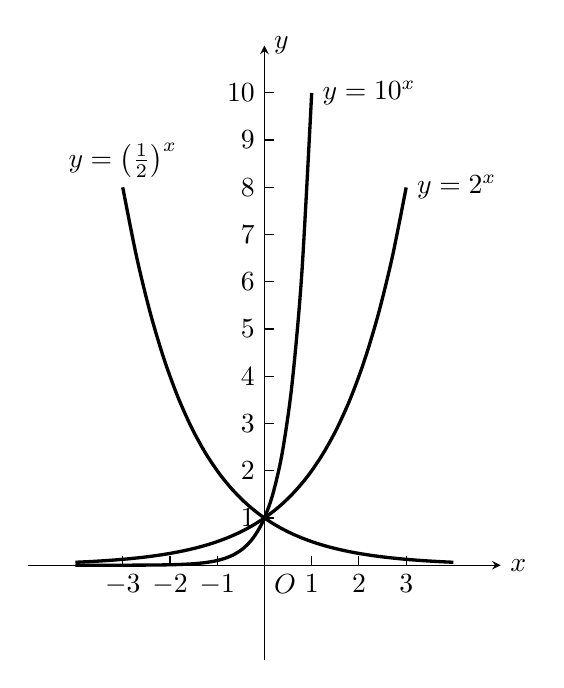
\begin{tikzpicture}[>=stealth, scale=.6]
 \draw[->](-5,0)--(5,0)node[right]{$x$};
 \draw[->](0,-2)--(0,11)node[right]{$y$};
 \foreach \x in {-3,-2,-1,1,2,3}
 {
     \draw(\x,0)node[below]{$\x$}--(\x,.2);
 }
 \foreach \x in{1,2,3,...,10}
 {
     \draw(0,\x)node[left]{$\x$}--(.2,\x);
 }
 \draw[domain=-4:1, smooth, very thick]plot(\x, 10^\x)node[right]{$y=10^x$};
 \draw[domain=-3:4, smooth, very thick]plot(\x, 0.5^\x);
 \node [below right]{$O$};
 \node at (-3,8)[above]{$y=\left(\frac{1}{2}\right)^x$};
 \draw[domain=-4:3, smooth, very thick]plot(\x, 2^\x)node[right]{$y=2^x$};
 
 
 \end{tikzpicture}
     \caption{}
 \end{figure}
 
 
 我们看到这些图象的共同点是:
 
 图象都在$x$轴上方,即对任何$x\in\R$,都有$y>0$;图象都通过$(0,1)$点,即当$x=0$时,恒有$y=a^0=1\; (0<a\ne 1)$,当$a>1$时,曲线以$x$轴负方向为渐近线,且当$x$增加时,曲线是上升的(即$y$是$\R$上的增函数);当$0<a<1$时,曲线以$x$轴正方向为渐近线,且当$x$增加时,曲线是下降的(即$y$是$\R$上的减函数)。
 
 我们还看到:$y=2^x$与$y=\left(\frac{1}{2}\right)^x$这样两个函数的图象关于$y$轴对称(这一点你能从理论上证明吗?)。
 
 \subsection{指数函数$y=a^x\; (0<a\ne 1)$的性质}
 列表如下:
 \begin{table}[htp]
     \caption{}
     \centering
 \begin{tabular}{c|cc}
     \hline
 $y=a^x$ & $a>1$&$0<a<1$        \\
 \hline
 定义域 & $\R$ & $\R$\\
 值域 & $(0,+\infty)$& $(0,+\infty)$\\
 &\multicolumn{2}{c}{任一正数$m$都能写成指数形式$m=a^x$}\\
 单调性& $y$是$\R$上的增函数& $y$是$\R$上的减函数\\
 & $a^x=\begin{cases}
     <1,& x<0\\
     =1,& x=0\\
     >1,& x>0
 \end{cases}$  & $a^x=\begin{cases}
     >1,& x<0\\
     =1,& x=0\\
     <1,& x>0
 \end{cases}$\\
 关键点&\multicolumn{2}{c}{$(0,1),\quad (1,a),\quad \left(-1,\frac{1}{a}\right)$}\\
 底数对图象的影响&\multicolumn{2}{c}{$y=a^x$与$y=\left(\frac{1}{a}\right)^x$的图象关于$y$轴对称}\\
 \hline
 \end{tabular}
 \end{table}
 
 \begin{center}
 \begin{tikzpicture}[>=stealth]
 \begin{scope}
 \draw[->](-2,0)--(2,0)node[right]{$x$};
 \draw[->](0,-1)--(0,4)node[right]{$y$};
 \node [below left]{$O$};
 
 \foreach \x in {1,2,3}
 {
     \draw(0,\x)--(-.1,\x)node[left]{$\x$};
 }
 \foreach \x in{-1,1}
 {
     \draw(\x,0)--(\x,-.1)node[below]{$\x$};
 }
 \draw[domain=-1.5:1.5, smooth, very thick]plot(\x, 2^\x)node[above]{$y=a^x$};
 \node at (1,1)[right]{$(a>1)$};
 \end{scope}
 \begin{scope}[xshift=6cm]
     \draw[->](-2,0)--(2,0)node[right]{$x$};
 \draw[->](0,-1)--(0,4)node[right]{$y$};
 \foreach \x in {1,2,3}
 {
     \draw(0,\x)--(-.1,\x)node[left]{$\x$};
 }
 \foreach \x in{-1,1}
 {
     \draw(\x,0)--(\x,-.1)node[below]{$\x$};
 }
 \draw[domain=1.5:-1.5, smooth, very thick]plot(\x, 0.5^\x)node[above]{$y=a^x$};
 \node at (-.5,1)[left]{$(0<a<1)$};
 \node [below left]{$O$};
 
 \end{scope}
 \end{tikzpicture}
 \end{center}
 
 \begin{note}
 \begin{enumerate}
     \item 在分析问题时,常常需要画出较正确的指数函数的
 草图。一般至少取三个点$(1,a)$、$(0,1)$与$\left(-1,\frac{1}{a}\right)$并且注意$x$轴是渐近线;
 \item 因为$y=a^x$的值域是$(0,+\infty)$,且在$\R$上$y$是$x$的单调函数,所以任意$m\in (0,\infty)$,都应找到唯一的$x_0$与之对应,即$m=a^{x_0}$。这就是说,\textbf{任一正数$m$都能写成指数形式};
 \item $a>1$时,由于$y=a^x$是$a$的增函数,且过$(0,1)$点,立刻可得
 \[a^x \begin{cases}
     <1,& x<0\\
     =1,& x=0\\
     >1,& x>1
 \end{cases}\]
 (从图象上看,这一点十分清楚!)
 
 这是一组十分重要的不等关系。连同$0<a<1$时的不等关系与之类似(见表3.2);
 \item 若$f(x)=a^x$,则$f(-x)=a^{-x}=\left(\frac{1}{a}\right)^x$,这说明由$y=a^x$的图象作关于$y$轴的对称变换立刻可得到$y=\left(\frac{1}{a}\right)^x$的图
 象。所以$y=a^x$与$y=\left(\frac{1}{a}\right)^x$的图象关于$y$轴对称。
 \end{enumerate}
 \end{note}
 
 \begin{example}
     一种放射性物质不断蜕变为其他物质,每过一年剩留质量约为原来的84\%,写出剩留质量$y$与经过的时间$x$(年)的关系式,并通过其函数图象求出约经过多少年剩留质量恰为原来的一半(结果保留一个有效数字).
 \end{example}
 
 \begin{solution}
    设最初的质量为1。经过1年,剩留质量是$y_1=1\times 4\%=0.84$,经过2年,剩留质量$y_2=0.84\times 84\%=0.84^2$, 经过$x$年,剩留质量$y_x=0.84^x\; (x\ge 0)$,这是一个指数函数,据此列表:
 \begin{center}
     \begin{tabular}{ccccccccc}
 \hline
 $x$&0&1&2&3&4&5&6&$\cdots$\\
 \hline
 $y$&1&0.84&0.71&0.59&0.50&0.42&0.35&$\cdots$ \\
 \hline
     \end{tabular}
 \end{center}
 用描点法画出函数的图象(图3.8)。因为这是一个减函数的图象[底数$a\in(0,1)$],从图上看出:要使$y=0.5$, $x=4$.
 \begin{figure}[htp]
     \centering
 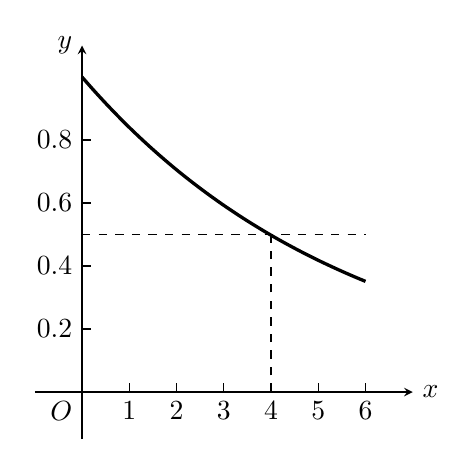
\begin{tikzpicture}[yscale=4, xscale=.6,>=stealth]
 \draw[->](-1,0)--(7,0)node[right]{$x$};
 \draw[->](0,-.15)--(0,1.1)node[left]{$y$};
 \foreach \x in {1,2,...,6}
 {
     \draw(\x,0)node[below]{$\x$}--(\x,.03);
 }
 \foreach \x in {0.2,0.4,0.6,0.8}
 {
     \draw(0,\x)node[left]{$\x$}--(.2,\x);
 }
 \draw[domain=0:6, smooth, very thick]plot(\x, 0.84^\x);
 \node [below left]{$O$};
 \draw[dashed](0,.5)--(6,.5);
 \draw[dashed](4,0)--(4,.5);
 
 \end{tikzpicture}
     \caption{}
 \end{figure}
 
 答:约过4年,剩留质量为原来之半。
 \end{solution}
 
 \begin{ex}
 由$y=2^x$的图象,你能简捷地作出下列函数的图象吗?
 \begin{multicols}{2}
 \begin{enumerate}[(1)]
     \item $y=2^{x+3}-1$
     \item $y=2^{x-3}+1$
     \item $y=4\cdot 2^x$
     \item $y=\left(\frac{1}{2}\right)^x$
     \item $y=-2^{x}$
     \item $y=2^{|x|}$
 \end{enumerate}
 \end{multicols}
 \end{ex}
 
 \begin{analyze}
     运用图象几何变换的方法(见2.9节)能简捷地作出这些函数的图象。
 \end{analyze}
 
 \begin{example}
     求出$y=2^{x+3}-1$与$y=2^{|x|}$的定义域、值域和单调区间。
 \end{example}
 
 \begin{solution}
 \begin{enumerate}[(1)]
     \item 由$y=2^x$的图象左移3个单位,再下移1个
     单位,可得到$y=2^{x+3}-1$的图象(图3.9).从而可知,$D=\R$,值域是$(-1,+\infty)$, 它的增区间是$(-\infty,+\infty)$。
     \item 因为$y=2^{|x|}$是偶函数,当$x\ge 0$时与$y=2^x\; (x\ge 0)$的图象重合。由对称性可作出$x<0$时的图象(图3.10).所以,$y=2^{|x|}$的定义域是$\R$,值域是$[1,+\infty)$, $(-\infty,0]$是减区间,$[0,+\infty)$是增区间。
 \end{enumerate}
 \begin{figure}[htp]
     \centering
 \begin{minipage}{.45\textwidth}
     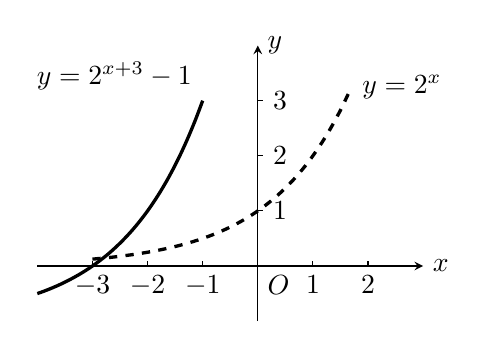
\begin{tikzpicture}[>=stealth, scale=.7]
 \draw[->](-4,0)--(3,0)node[right]{$x$};
 \draw[->](0,-1)--(0,4)node[right]{$y$};
 \draw[domain=-4:-1, smooth, very thick]plot(\x, 8*2^\x -1)node[above left]{$y=2^{x+3}-1$};
 \draw[domain=-3:1.7, smooth, dashed, very thick]plot(\x, 2^\x)node[right]{$y=2^{x}$};        
 \node [below right]{$O$};
 \foreach \x in {-3,-2,-1,1,2}
 {
     \draw(\x,0)node[below]{$\x$}--(\x,.1);
 }
 \foreach \x in{1,2,3}
 {
     \draw(0,\x)--(.1,\x)node[right]{$\x$};
 }
 
     \end{tikzpicture}
 \caption{}    
 \end{minipage}
 \hfill
 \begin{minipage}{.45\textwidth}
 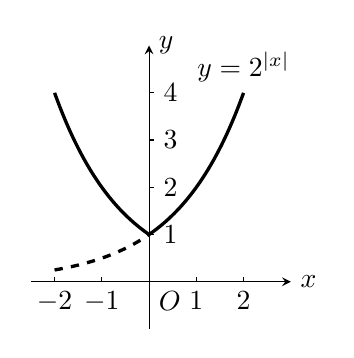
\begin{tikzpicture}[>=stealth, scale=.6]
     \draw[->](-2.5,0)--(3,0)node[right]{$x$};
     \draw[->](0,-1)--(0,5)node[right]{$y$};
     \draw[domain=0:2, smooth, very thick]plot(\x, 2^\x)node[above]{$y=2^{|x|}$};
     \draw[domain=0:2, smooth, very thick]plot(-\x, 2^\x);
     \draw[domain=-2:0, smooth, dashed, very thick]plot(\x, 2^\x);
     \node [below right]{$O$};
     \foreach \x in {-2,-1,1,2}
     {
         \draw(\x,0)node[below]{$\x$}--(\x,.1);
     }
     \foreach \x in{1,2,3,4}
     {
         \draw(0,\x)--(.1,\x)node[right]{$\x$};
     }
 \end{tikzpicture}
     \caption{}    
     \end{minipage}
 \end{figure}
 
 
 \end{solution}
 
 \begin{example}
     比较下列每题中两个数的大小。
 \begin{multicols}{2}
 \begin{enumerate}[(1)]
     \item $0.6^{-2.1}$与$0.8^{- 2.1}$
     \item $( 2\sqrt 2) ^{\tfrac 13}$与$\left(\frac7{18}\right)^{-\tfrac{1}{3}}$
     \item $1.7^{-2.5}$与$1.7^{-2.1}$
     \item $0.9^{0.1}$与$0.9^{0.2}$
 \end{enumerate}
 \end{multicols}
 \end{example}
 
 \begin{analyze}
     (1)、(2)题是“同指数”的幂,可利用幂函数
 的单调性比大小,(3)、(4)题是“同底数”的幂,可利用指数函数的单调性比大小。
 \end{analyze}
 
 \begin{solution}
 \begin{enumerate}[(1)]
     \item $\because \quad $幂函数 $y=x^{-2.1}\; (x>0)$单调递减,且$0.6<0.8$,
     
 $\therefore\quad 0.6^{-2.1}>0.8^{-2.1}$    
 
 \item $\because\quad $幂函数$y=x^{\tfrac13}\; (x>0)$单调递增,且
 $2\sqrt{2}<\frac{18}{7}$,
 
 $\therefore\quad ( 2\sqrt 2) ^{\tfrac 13}<\left(\frac7{18}\right)^{-\tfrac{1}{3}}$
 
 \item $\because \quad $指数函数$y=1.7^x$单调递增,且$-2.5<-2.1$,
 
 $\therefore\quad 1.7^{-2.5}<1.7^{-2.1}$
 
 \item $\because \quad $指数函数$y=0.9^x$单调递减,且$0.1<0.2$,
 
 $\therefore\quad 0.9^{0.1}>0.9^{0.2}$
 \end{enumerate}
 \end{solution}
 
 \begin{example}
     比较下列各题中两个数的大小:
 \begin{multicols}{2}
 \begin{enumerate}[(1)]
     \item $2.6^{3.2}$与$\left ( \frac 1{\sqrt {5}}\right ) ^{- 3.2} $, 
     \item $1.8^{3.4}$与$3^{1.7}$,
     \item $\left(\frac7{10}\right)^{-0.81}$与$\left(1\frac37\right)^{0.92}$,
     \item $1.7^{0.3}$与$0.9^{3.1}$
 \end{enumerate}
 \end{multicols}
 \end{example}
 
 \begin{analyze}
     这些幂既不同指数,又不同底数,但除(4)以
 外,有的能化成“同底”,有的能化成“同指”。
 \end{analyze}
 
 \begin{solution}
 \begin{enumerate}[(1)]
     \item $\because\quad \left(\frac{1}{\sqrt{5}}\right)^{-3.2}=(\sqrt{5})^{3.2}$,幂函数$y=x^{3.2}\; (x>0)$单调递增,且$2.6>\sqrt{5}$,
     
 $\therefore\quad 2.6^{3.2}>\left ({\sqrt {5}}\right ) ^{3.2}\Longrightarrow 2.6^{3.2}>\left ( \frac 1{\sqrt {5}}\right ) ^{- 3.2}$
 
 \item $\because\quad 3^{1.7}=\left(\sqrt{3}\right)^{3.4}$,幂函数$y=x^{3.4}\; (x>0)$单调递增,且$1.8>\sqrt{3}$,
 
 $\therefore\quad 1.8^{3.4}>\left ({\sqrt {3}}\right ) ^{3.4}\Longrightarrow 1.8^{3.4}>3^{1.7}$.
 
 \item $\because\quad \left(1\frac{3}{7}\right)^{0.92}=\left(\frac{7}{10}\right)^{-0.92}$,指数函数$y=\left(\frac{7}{10}\right)^x$单调递减,且$-0.81>-0.92$,
 
 $\therefore\quad \left(\frac{7}{10}\right)^{-0.81}<\left(\frac{7}{10}\right)^{-0.92}\Longrightarrow \left(\frac{7}{10}\right)^{-0.81}<\left(1\frac{3}{7}\right)^{0.92}$.
 
 \item 分析:因为$1.7^{0.3}$与$0.9^{3.1}$既不“同底”,也不“同
 指”,又化不成“同底”或“同指”。所以,不能直接利用某个指数函数(或幂函数)的单调性比大小。现在考虑能否在这两个数值之间寻找一个中间值,使它比其中一个数大,而比另外一个数小.
 
 \textbf{方法1:} 由指数函数的单调性,有
 \[1.7^{0.3}>1.7^0=1,\qquad 0.9^{3.1}<0.9^0=1\]
 即:$1.7^{0.3}>1,\quad 0.9^{3.1}<1$\hfill (图3.11)
 
 $\therefore\quad 1.7^{0.3}>0.9^{3.1}$.
 
 \textbf{方法2:} 由幂函数的单调性,有
 \[1.7^{0.3}>1^{0.3}=1,\qquad 0.9^{3.1}<1^{3.1}=1\]
 即
 $1.7^{0.3}>0.9^{3.1}$\hfill (图3.12)
 \end{enumerate}
 \end{solution}
 
 \begin{figure}[htp]
     \centering
 \begin{minipage}{.45\textwidth}
 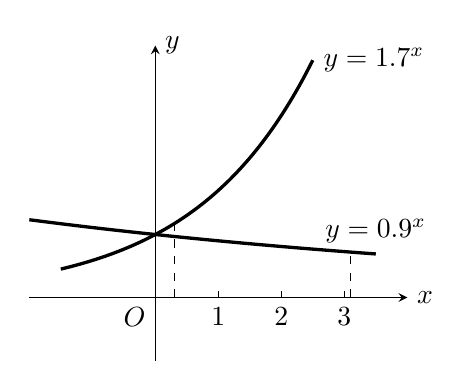
\begin{tikzpicture}[scale=.8, >=stealth]
    \draw[->](-2,0)--(4,0)node[right]{$x$};
 \draw[->](0,-1)--(0,4)node[right]{$y$};
 \node [below left]{$O$};
 \draw[domain=-1.5:2.5, smooth, very thick]plot(\x, 1.7^\x)node[right]{$y=1.7^x$};
 \draw[domain=-2:3.5, smooth, very thick]plot(\x, 0.9^\x)node[above]{$y=0.9^x$}; 
 \draw[dashed](0.3,0)--(0.3,1.7^0.3);
 \draw[dashed](3.1,0)--(3.1,0.9^3.1);
 \foreach \x in {1,2,3}
 {
     \draw(\x,0)node[below]{\x}--(\x,.1);
 }
 
 \end{tikzpicture}
 \caption{}
 \end{minipage}\hfill
 \begin{minipage}{.45\textwidth}
 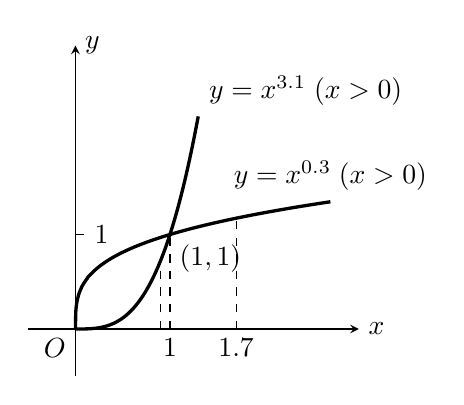
\begin{tikzpicture}[scale=1.2, >=stealth]
     \draw[->](-.5,0)--(3,0)node[right]{$x$};
 \draw[->](0,-.5)--(0,3)node[right]{$y$};
 \node [below left]{$O$};    
 \draw[domain=0:1.3, smooth, very thick, samples=100]plot(\x, \x^3.1)node[above right]{$y=x^{3.1}\; (x>0)$};
 \draw[domain=0:2.7, smooth, very thick, samples=1000]plot(\x, \x^0.3)node[above]{$y=x^{0.3}\; (x>0)$}; 
 \draw[dashed](1,0)node[below]{1}--(1,1)node[below right]{$(1,1)$};
 \draw[dashed](0,1)--(.1,1)node[right]{1};
 \draw[dashed](1.7,0)node[below]{1.7}--(1.7,1.7^0.3);
 \draw[dashed](0.9,0)--(0.9,0.9^3.1);
 
 
 \end{tikzpicture}
 \caption{}
 \end{minipage}
 \end{figure}
 
 
 
 
 \begin{note}
 (1)、(2)、(3)题是把要比大小的幂“转化”为同底幂或同指数幂加以处理。第(4)题方法的实质是在要比大小的两个幂之间搭一个桥(找一个中间值),间接达到比大小的目的,这种方法不妨称为中间值法(也是一种有用的思考方法).本题在寻找中间值的过程中,利用了指数函数的关键点$(0,1)$与幂函数的关键点$(1,1)$附近的函数的性质.
 \end{note}
 
 \begin{example}
 解不等式:\begin{multicols}{2}    
 \begin{enumerate}[(1)]
     \item $a^{2x^2-7x+3}>1\; (a>1)$
     \item $a^{2x^2-3x+1}>a^{x^2+2x-5}\; (0<a<1)$
 \end{enumerate}
 \end{multicols}
 \end{example}
 
 \begin{solution}
 \begin{enumerate}[(1)]
     \item 原不等式可写成
 $$a^{2x^2-7x+3}>a^0\quad (a>1)$$
 因为$a>1$时$y=a^{u}$单调递增,由上式可得
 \begin{equation}
   2x^2-7x+3>0  \tag{*}
 \end{equation}
 解(*), 得$x<\frac{1}{2}$或$x>3$,
 
 $\therefore \quad (1)$ 的解集为$\left ( - \infty, \frac 12\right ) \cup ( 3, + \infty) $
 
 \item 当$0<a<1$时,$y=a^u$单调递减,由(2)得
 $$2x^{2}-3x+1<x^{2}+2x-5$$
 整理,得
 \begin{equation}
     x^{2}-5x+6<0 \tag{**}   
 \end{equation}
 解(**), 得$2<x<3$,
 
 $\therefore\quad $(2)的解集为$(2,3)$.
 \end{enumerate}
 \end{solution}
 
 \subsection{简单复合函数的单调性}
 设$y=f(u)$, $u=g(x)$。若$u=g(x)$在$[a,b]$上是单调函数,$y=f(u)$在区间$[g(a), g(b)]$或$[g(b), g(a)]$上也是单调函数,那么$y=f[g(x)]$在$[a,b]$上一定是单调函数,且具体分为以下四种情况:
 
 \begin{center}
 \begin{tabular}{c|ccc}
 \hline
 & $u=g(x)$& $y=f(u)$& $y=f[g(x)]$\\
 \hline
 情况1&增&增&增\\
 情况2&增&减&减\\
 情况3&减&增&减\\
 情况4&减&减&增\\
 \hline
 \end{tabular}
 \end{center}
 
 \begin{note}
 若$u=g(x)$单调递增,则较大的$x$必对应较大的$u$;且$y=f(u)$单调递增,则较大的$u$必对应较大的$y$ $\Longrightarrow $较大的$x$必对应较大的$y$
 
 $\therefore\quad y$是$x$的增函数(情况1)。其余情况类似。
 \end{note}
 
 \begin{example}
     求函数$y=a^{-2x^2-8x+1}\quad (0<a<1)$ 的单调增区间。
 \end{example}
 
 \begin{solution}
     这个函数可看作是由
 $y=a^u\; (0<a<1)$ 与
 $u=-2x^2-8x+1$
 复合而成的。由于函数$y=a^u\; (0<a<1)$在$\R$上是减函数,据复合函数的单调性,欲使$y=a^{-2x^2-8x+1}$是增函数,只要使$u=-2x^2-8x+1$为减函数。
 
 $\because\quad $二次项系数$-2<0$,$x_0=\frac{-(-8)}{2(-2)}=-2$
 
 $\therefore\quad [-2,+\infty)$是$u=-2x^2-8x+1$的减区间。从而$y=a^{-2x^2-8x+1}\; (0<a<1)$的单调增区间是$[-2,+\infty)$.
 \end{solution}
 
 \section*{习题二}
 \begin{center}
     \bfseries A
 \end{center}
 
 \begin{enumerate}
     \item 在同一坐标系内,画出下列三个函数的图象
 \begin{multicols}{3}
 \begin{enumerate}[(1)]
     \item $y=3^x$
     \item $y=\left(\frac{1}{3}\right)^x$
     \item $y=2^x$
 \end{enumerate}
 \end{multicols}
 
 \item 证明:在同一坐标系中,两个指数函数$y=a^x$与$y=\left(\frac{1}{a}\right)^x\; (0<a\ne 1)$的图象关于$y$轴对称。
 \item 一片树林中现有木材30000米$^3$,如果每年增长5\%,经过
 $x$年,树林中有木材$y$米$^3$,写出$x$,$y$间的函数关系式,并且利用图象求约经过多少年,木材可以增加到40000米$^3$(结果保留一个有效数字)。
 \item \begin{enumerate}[(1)]
     \item 一种产品的年产量原来是$a$件,在今后$m$年内,计划使年产量平均每年比上一年增产$p\%$,写出年产量随经过年数变化的函数关系式。
     \item 一种产品的成本原来是$a$元,在今后$m$年内,计划使成本平均每年比上一年降低$p\%$,写出成本随经过年数变化的函数关系式。
 \end{enumerate}
 \item 目前我国人口总数是11亿,人均占有粮食是360千克。
 \begin{enumerate}[(1)]
     \item 如果人口平均每年增长2\%,粮食总产量平均每年增长4\%。那么,几年后人均一年占有500千克粮食(只列出方程,不用解)?
     \item 如果粮食总产量的年增长率是4\%,要想10年达到人均一年占有500千克粮食,那么,人口年增长率需要控制在什么水平上(只列出方程,不用解)?
 \end{enumerate}
 
 \item 求下列函数的定义域与值域: 
 \begin{multicols}{3}
 \begin{enumerate}[(1)]
     \item $y=3^{2-3x}$
     \item $y=2^{3x+1}-3$
     \item $y=\left(\frac{1}{2}\right)^{3x}+1$
     \item $y=4^{|x|}$
     \item $y=2^{3+|x|}$
     \item $y=2^{|x-3|}$
 \end{enumerate}
 \end{multicols}
 
 \item 比较下列各题中两个值的大小:
 \begin{multicols}{2}
 \begin{enumerate}[(1)]
     \item $2^{-0.6}$与$2^{0.6}$
     \item $0.32^{-0.2}$与$0.32^{0.2}$
     \item $0.99^{3.2}$与$0.99^{5.5}$
     \item $7.8^{-5}$与$7.8^{-7}$
     \item $5.5^{2.4}$与$6.6^{2.4}$
     \item $0.78^{-\tfrac{1}{3}}$与$0.80^{-\tfrac{1}{3}}$
     \item $3.2^{-6.8}$与$\left(\sqrt{3}\right)^{6.8}$
     \item $7.1^{1.8}$与$1.6^{0.9}$
     \item $\left(\frac{2}{3}\right)^{-0.2}$与$1.5^{0.4}$
     \item $\left(\frac{2}{3}\right)^{3.2}$与$\left(1\frac{1}{3}\right)^{-0.3}$
 \end{enumerate}
 \end{multicols}
 
 \item 讨论函数$y=\left(\frac{2}{3}\right)^{3x^2-5x-1}$的增减性。
 \item 解下列不等式:
 \begin{enumerate}[(1)]
     \item $3^{x^2-6x-16}<1$
     \item $4^{x^2+6x+16}>4^{2x^2+6x}$
     \item $a^{2x^2+3x+1}\ge a^{x^2-x-2}\; (0<a<1)$
 \end{enumerate}
 
 \item 设$y_1=a^{3x^2+8x}$, $y_2=a^{3x+2}$,其中$0<a\ne 1$,试求当$x$为何值时有$y_1<y_2$.
 \item 设$f(x)=10^x$,求证:
 \begin{multicols}{2}
 \begin{enumerate}[(1)]
     \item $f(x)\cdot f(y)=f(x+y)$
     \item $f(x)\div f(y)=f(x-y)$
 \end{enumerate}
 \end{multicols}
 
 \item 求证:
 \begin{enumerate}[(1)]
     \item $f(x)=\frac{a^x-a^{-x}}{2}\quad (0<a\ne 1)$是奇函数。
     \item $g(x)=x\cdot \frac{a^x-1}{a^x+1}\quad (0<a\ne 1)$是偶函数。
 \end{enumerate}
 \end{enumerate}
 
 \section{对数}
 \subsection{什么是对数}
 在研究指数函数性质的时候,我们已经知道:任何一个正数$m$都能写成指数形式,为了简捷地计算出
 \[\frac{35\cdot 145}{\sqrt[3]{20^2\cdot 157}}\]
 的值$y_0$,可用下面的办法。
 
 \begin{figure}[htp]
     \centering
 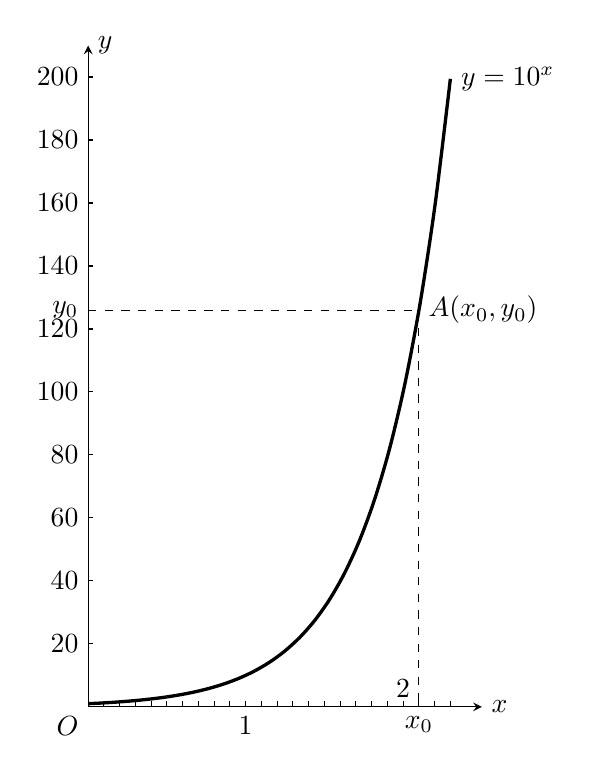
\begin{tikzpicture}[yscale=.04, xscale=2, >=stealth]
 \draw[->](0,0)--(2.5,0)node[right]{$x$};
 \draw[->](0,0)--(0,210)node[right]{$y$};
 \draw[domain=0:2.3, very thick, smooth]plot(\x, 10^\x)node[right]{$y=10^x$};
 \foreach \x in {20,40,...,200}
 {
     \draw(0,\x)node[left]{\x}--(.03,\x);
 }
 \node at (1,0)[below]{1};
 \node at (2,0)[above]{2};
 \node [below left]{$O$};
 \foreach \x in {.1,.2,...,2.3}
 {
     \draw(\x,0)--(\x,2);
 }
 \draw[dashed](0,126)node[left]{$y_0$}--(2.1,126)node[right]{$A(x_0,y_0)$}--(2.1,0)node[below]{$x_0$};
 
 \end{tikzpicture}
     \caption{}
 \end{figure}
 
 
 利用指数函数$y=10^x$的图象(图3.13),可以把上式中有关的数写成指数形式:
 \[35\approx 10^{1.54},\quad 145\approx 10^{2.16},\quad 
 20\approx 10^{1.80},\quad 157\approx 10^{2.20}\]
 那么
 \[y_0\approx \frac{10^{1.54}\cdot 10^{2.16}}{\sqrt[3]{10^{2\times 1.80}\cdot 10^{2.20}}}\]
 再回到图3.13,可以看出当$x_0\approx 2.10$时,$y_0\approx 126$.
 
 这种办法简捷就在于:它用幂的指数的加、减、乘、除运算分别替代了原来数字的乘、除、乘方、开方运算。办法得以实施的条件是把有关的数写成了指数形式(幂的形式),
 \begin{center}
 \begin{tikzpicture}[>=stealth, thick]
     \node at (0,0){\huge $145=10^{2.16}$};
 \node at (3,-1)[right]{幂的底数};
 \node at (3,1)[right]{幂的指数};
 \draw[->](3,1)--(1.5,1)--(1.5,0.5);
 \draw[->](3,-1)--(0.5,-1)--(0.5,-.5);
 
 \end{tikzpicture}
 \end{center}
 如这里,幂的指数2.16又称为以10为底145的对数。一般有下面的定义
 
 \begin{thm}{定义}
 设$a>0$,且$a\ne 1$,对于数$N$,若能找到实数$x$,使得
 \begin{equation}
     N=a^x\tag{1}
 \end{equation}
 那么,数$x$就称为\textbf{以$a$为底$N$的对数}\footnote{$\log_a N$是英语“logarithm(对数) of $N$”的缩写。},记作
 \begin{equation}
     x=\log_a N \tag{2}
 \end{equation}
 其中$a$叫做\textbf{底数}(简称\textbf{底}),$N$叫做\textbf{真数}。
 \end{thm}
 
 \begin{note}
 \begin{enumerate}
     \item 以$a\; (0<a\ne 1)$为底,数$N$存在对数的充要条件是能找到实数$x$,使(1)式成立;
     \item (1)式中的$x$具有双重身份:既是幂的指数,又是以$a$为底,数$N$的对数。通常称(1)为\textbf{指数式},(2)为\textbf{对数式}。
     
     指数式中的底数、指数、幂与对数式中的底数、对数、真数的对应关系如图3.14:
 
 \item 从对数的定义可以看出:“对数源于指数”。这是大数学家欧拉(Euler)的名言,是对对数本质的高度概括,对学习对数具有指导意义。因此,某些对数问题(如对数的性质及运算法则等)往往都要通过指数来解决。
 \end{enumerate}
 \end{note}
 
 \begin{blk}
 \begin{enumerate}[(1)]
     \item 零和负数存在对数吗?为什么?
     \item 你能证明下列两个重要的对数恒等式吗?
 \[\log_a a^k=k\; (k\in\R),\qquad a^{\log_a m}=m\; (m>0)\]
 其中:$0<a\ne 1$.
 (特例:$\log_a a=1,\quad \log_a 1=0$)
 \end{enumerate}
 
 \end{blk}
 
 
 \begin{figure}[htp]
     \centering
 \begin{tikzpicture}[>=stealth]
 
 \node[draw, rectangle] at (-3,0){\huge $a^b=N$};
 \node[draw, rectangle] at (3,0){\huge $\log_a N=b$};
 \draw[<->, thick](-4,-.5)--(-4,-1.5)--node[fill=white]{底数}(2.4,-1.5)--(2.4,-.5);
 \draw[<->, thick](-3.6,.5)--(-3.6,1.5)--node[fill=white]{指数\quad 对数}(4.6,1.5)--(4.6,.5);
 \draw[<->, thick](-2.1,.5)--(-2.1,.8)--node[fill=white]{幂\quad\quad 真数}(3,.8)--(3,.5);
 \draw[dashed](.5,0)--(.5,3);
 \node at (-1,2.5){指数式};
 \node at (2,2.5){对数式};
 
 \end{tikzpicture}
     \caption{}
 \end{figure}
 
\begin{example}
\begin{enumerate}[(1)]
    \item 已知$\log_{10}N=-2$, 求$N$,
    \item 已知$\log_2 M=5$, 求$M$.
\end{enumerate}
\end{example}
 

\begin{solution}
\begin{enumerate}[(1)]
    \item 由$\log_{10}N=-2$, 得$N=10^{-2}=\frac{1}{10^{2}}=\frac{1}{100}$.
    \item 由$\log _2M= 5$, 得 $M= 2^5= 32$
\end{enumerate}
\end{solution}
 
\begin{multicols}{2}
    \begin{example}
    求下列各式的值:
\begin{enumerate}[(1)]
    \item $\log_9 81$,
    \item $\log_3\frac 1{27}$,
    \item $\log_{10} 1000$.
\end{enumerate}    

\end{example}
 
\begin{solution}
\begin{enumerate}[(1)]
    \item $\log_{3}81=\log_9 9^2=2$
    \item $\log_3\frac 1{27}=\log_{3}3^{- 3}= - 3$
\item $\log_{10}1000=\log_{10}10^3=3$
\end{enumerate}
\end{solution} 
\end{multicols}


\begin{rmk}
    此例也可以先化成指数式来解。如(1): 
    设$\log_9 81=x$,则$9^x=81$,

$\because\quad 9^2=81$

$\therefore\quad x=2\Longrightarrow \log_9 81=2$
\end{rmk}

\begin{multicols}{2}
\begin{example}
    求下列各式的值:
\begin{enumerate}[(1)]
    \item $\log_4 4$
    \item $\log_3 1$
\end{enumerate}
\end{example}
 
\begin{solution}
    \begin{enumerate}[(1)]
        \item $\log_4 4=\log_4 4^1=1$
        \item $\log_3 1=\log_3 3^0=0$
    \end{enumerate}
\end{solution}    
\end{multicols}


\begin{example}
    求下列各式的值:
    \begin{multicols}{3}
\begin{enumerate}[(1)]
    \item $2^{\log_2 3}$
    \item $2^{3\log_2 3}$
    \item $2^{-\tfrac{1}{2}\log_2 3}$
\end{enumerate}
\end{multicols}
\end{example}
 
\begin{solution}
\begin{enumerate}[(1)]
    \item $2^{\log_2 3}=3$
    \item $2^{3\log_2 3}=\left(2^{\log_2 3}\right)^3=3^3=27$
    \item $2^{-\tfrac{1}{2}\log_2 3}=\left(2^{\log_2 3}\right)^{-\tfrac{1}{2}}=3^{-\tfrac{1}{2}}=\frac{\sqrt{3}}{3}$
\end{enumerate}
\end{solution}    

\begin{ex}
\begin{enumerate}
    \item 把下列指数式写成对数式:
\begin{multicols}{3}
\begin{enumerate}[(1)]
    \item $2^4=16$
    \item $5^{-2}=\frac{1}{25}$
    \item $10^4=10000$
    \item $10^0=1$
    \item $8^{\tfrac{2}{3}}=4$
    \item $27^{-\tfrac{1}{3}}=\frac{1}{3}$
\end{enumerate}
\end{multicols}
    \item 把下列对数式写成指数式:
\begin{multicols}{2}
    \begin{enumerate}[(1)]
        \item $\log_4 16=2$
        \item $\log_3\frac{1}{81}=-4$
        \item $\log_8 2=\frac{1}{3}$
        \item $\log_{10}0.0001=-4$
        \item $\log_7 7 =1$
        \item $\log_{81} 3=\frac{1}{4}$
        \item $\log_{27}\frac{1}{9}=-\frac{2}{3}$
        \item $\log_{\tfrac{1}{5}}125=-3$
    \end{enumerate}
\end{multicols}
    \item 求下列各式的值:
\begin{multicols}{3}
    \begin{enumerate}[(1)]
\item $\log_4 64$
\item $\log_2 \frac{1}{16}$
\item $\log_3 243$
\item $\log_{10}0.0001$
\item $\log_{\tfrac{1}{5}}625$
    \end{enumerate}
\end{multicols}
    \item 求下列对数式中的真数$x$:
\begin{multicols}{2}
    \begin{enumerate}[(1)]
        \item $\log_3 x=3$
        \item $\log_{\tfrac{1}{2}} x=-3$
        \item $\log_5 x=1$
        \item $\log_4 x=0$
    \end{enumerate}
\end{multicols}
    \item 求下列各式的值:
\begin{multicols}{3}
    \begin{enumerate}[(1)]
        \item $\log_{15}15 $
        \item $\log_{0.4}1 $
        \item $\log_{\tfrac{1}{3}}9 $
        \item $\log_{3} 1$
        \item $\log_{3.6} 3.6$
        \item $\log_{2} 1024$
    \end{enumerate}
\end{multicols}
    \item 求下列各式的值:
    \begin{multicols}{3}
        \begin{enumerate}[(1)]
            \item $7^{\log_7 5}$
            \item $3^{-2\log_3 5}$
            \item $\left(\frac{1}{2}\right)^{-\log_2 3}$
            \item $4^{-\log_2 3}$
            \item $5^{-\tfrac{2}{3}\log_5 4}$
            \item $125^{-2\log_5 2}$
        \end{enumerate}
\end{multicols}
\end{enumerate}    
\end{ex} 
 
\subsection{正数的积、商、幂、方根的对数}

我们知道,指数运算有下列法则:
\[\begin{split}
a^p\cdot a^q&=a^{p+q}\\
a^p\div a^q&=a^{p-q}\\
(a^p)^n&=a^{np}\\
\sqrt[n]{a^p}&=a^{\tfrac{p}{n}}\\
\end{split}\qquad \text{(其中$0<a\ne 1$, 
$p,q\in\R$, $n\in \N$.)}\]

现在研究正数的积、商、幂、方根的对数如何计算?先
看
\[\log_a (M\cdot N)=?\quad (0<a\ne 1,\; M>0,\; N>0)\]
由于“对数源于指数”,因而只要把$(M\cdot N)$
改写成以$a$为底的指数形式就可以了。

由对数恒等式知
\begin{equation}
    M=a^{\log_a M},\qquad N=a^{\log_a N} \tag{*}
\end{equation}
于是
\[\begin{split}
    \log_a(M\cdot N)&=\log_a\left(a^{\log_a M}\cdot a^{\log_a N}\right)\\
    &=\log_a a^{\log_a M+\log_a N}\\
    &=\log_a M+\log_a N
\end{split}\]

这就是说,\textbf{两个正数的积的对数,等于同一底数的这两
个数的对数的和},即
\[\log_a MN=\log_a M+\log_a N\]

当因数多于两个时,上述性质仍然成立。例如
\[\log_a LMN=\log_a L+\log_a M+\log_a N\]
同理还可得出:

\textbf{两个正数的商的对数,等于同一底数的被除数的对数减
去除数的对数的差},即
\[\log_a \frac{M}{N}=\log_a M-\log_a N\]

\textbf{一个正数的幂的对数,等于幂的底数的 对数乘以幂指
数},即
\[\log_a M^n=n\log_a M\]

\textbf{一个正数的算术根的对数,等于被开方数的对数除以根
指数},即
\[\log_a\sqrt[n]{M}=\frac{1}{n}\log_a M\]

同学们可以自己证明这些性质。

\begin{example}
用$\log_a x$, $\log_a y$, $\log_a z$表示下列各式:
\begin{multicols}{2}
\begin{enumerate}[(1)]
    \item $\log_a \frac{xy}{z}$
    \item $\log_a (x^3\cdot y^5)$
    \item $\log_a \frac{\sqrt{x}}{yz}$
    \item $\log_a \frac{x^2\sqrt{y}}{\sqrt[3]{z}}$
\end{enumerate}
\end{multicols}
\end{example}

\begin{solution}
\begin{enumerate}[(1)]
    \item $\log_a \frac{xy}{z}=\log_a(xy)-\log_a z=\log_a x+\log_a y-\log_a z$
    \item $\log_a (x^3\cdot y^5)=\log_a x^3+\log_a y^5=3\log_a x+5\log_a y$
    \item $\log_a \frac{\sqrt{x}}{yz}=\log_a\sqrt{x}-\log_a(yz)=\frac{1}{2}\log_a x-\log_a y-\log_a z$
    \item $\log_a \frac{x^2\sqrt{y}}{\sqrt[3]{z}}=\log_a \left(x^2\cdot \sqrt{y}\right)-\log_a\sqrt[3]{z}=2\log_a x+\frac{1}{2}\log_a y-\frac{1}{3}\log_a z$
\end{enumerate}
 \end{solution}
 
\begin{example}
计算:
\begin{multicols}{2}
    \begin{enumerate}[(1)]
        \item $\log_{10}\sqrt[5]{100}$
        \item $\log_2 (4^7\cdot 2^5)$
    \end{enumerate}
\end{multicols}

\end{example}
 
\begin{solution}
    \begin{enumerate}[(1)]
        \item $\log_{10}\sqrt[5]{100}=\frac{1}{5}\log_{10}100=\frac{1}{5}\log_{10}10^2=\frac{2}{5}$
        \item $\log_2 (4^7\cdot 2^5)=7\log_2 4+5\log_2 2=14+5=19$
    \end{enumerate}
\end{solution}

\begin{ex}
\begin{enumerate}
    \item 证明公式
\[\log_a \sqrt[n]{M}=\frac{1}{n}\log_a M\quad (0<a\ne 1,\; M>0,\; n\in \N)\]
\item 用$\log_a x$, $\log_a y$, $\log_a z$, $\log_a (x+y)$, $\log_a (x-y)$表示下列各式:
\begin{multicols}{2}
\begin{enumerate}[(1)]
    \item $\log_a \frac{\sqrt{x}}{y^2 z}$
    \item $\log_a \left(x\cdot \sqrt[4]{\frac{z^3}{y^2}}\right)$
    \item $\log_a \left(xy^{\tfrac{1}{3}}z^{-\tfrac{2}{3}}\right)$
    \item $\log_a \frac{xy}{x^2-y^2}$
    \item $\log_a \left(\frac{x+y}{x-y}\cdot y\right)$
    \item $\log_a \left[\frac{y}{x(x-y)}\right]^3$
\end{enumerate}
\end{multicols}

\item 计算:    
\begin{multicols}{2}
\begin{enumerate}[(1)]
    \item $\log_a 2+\log_a \frac{1}{2}$
    \item $\log_3 18-\log_3 2$
    \item $2\log_5 10+\log_5 0.25$
    \item $\log_{10}\frac{1}{4}-\log_{10}25 $
\end{enumerate}
\end{multicols}
 
\item \begin{enumerate}[(1)]
    \item 用$a=\log_{10}5$表示$\log_{10}2$, $\log_{10}20$;
    \item 用$a=\log_{10}2$, $b=\log_{10}3$表示$\log_{10}4$, $\log_{10}5$, $\log_{10}6$, $\log_{10}15$.
\end{enumerate}
\end{enumerate}
\end{ex}
 
\subsection{常用对数}
通常我们用的是十进制记数法,所以通常用的对数也是
以10为底的对数,这种对数叫做\textbf{常用对数}。在表示常用对数
的时候,常常把底数10略去,并把
“log”
简写成“
“lg”
。如$\log_{10}M$可写作$\lg M$, $\log_{10}8$可写作$\lg8$. 一般所说的对数如不
做特殊说明,都是指常用对数。

常用对数当然具有一般对数所具有的通性(如上述对数
恒等式和积、商、幂、方根取对数的法则)。此外,常用对数
还有一些特殊的性质。

我们知道:
\begin{center}
\begin{tabular}{p{.4\textwidth}p{.4\textwidth}}
$\cdots\cdots$&$\cdots\cdots$\\
$10^3=1000$ & $\lg 1000=3$\\
$10^2=100$ & $\lg 100=2$\\
$10^1=10$ & $\lg 10=1$\\
$10^0=1$ & $\lg 1=0$\\
$10^{-1}=0.1$ & $\lg 0.1=-1$\\
$10^{-2}=0.01$ & $\lg 0.01=-2$\\
$10^{-3}=0.001$ & $\lg 0.001=-3$\\
$\cdots\cdots$&$\cdots\cdots$\\
\end{tabular}
\end{center}

可以看出,10的整数次幂的对数是一个整数,并且真数
较大的时候,它的对数也较大。

可以推断:
由$1<7.2<10$
,得$\lg1<\lg7.2<\lg10$,即
$0<\lg7.2<1$; 由$0.01<0.072<0.1$,得
$\lg0.01<\lg0.072<\lg0.1$,即
$-2<\lg0.072<-1$; ……

由此,\textbf{真数若不是10的整数次幂,则它的常用对数一定
是个小数}。特别,\textbf{若真数$\in (1,10)$, 则它的常用对数一定
是个正的纯小数}(这个纯小数可以从《对数表》查得)。

我们再考察$3.408$, $34.08$, $340.8$, $0.03408$以及
$0.0003408$的常用对数有什么关系?

由上可知,$\lg3.408$是个正的纯小数,查《对数表》可
得:$\lg3.408=0.5325$

$\because\quad 34.08=3.408\times10$

$\therefore\quad \lg34.08=\lg(3.408\times10)=\lg3.408+1=1+0.5325$

同理
\[\begin{split}
\lg340.8&=\lg(3.408\times10^{2})=\lg3.408+2=2+0.5325\\
\lg0.03408&=\lg(3.408\times10^{-2})=\lg3.408+(-2)
=-2+0.5325\\
\lg0.0003408&=\lg(3.408\times10^{-4})=\lg3.408+(-4)=-4+0.5325.
\end{split}\]

由此可见:
\begin{enumerate}[(1)]
    \item 若真数不是10的整数次幂,则它的常用对数一定
    可以写成一个整数(正整数,零或负整数)加上一个正的纯
    小数。其中整数部分叫做这个对数的首数,正的纯小数(或
    者为零)部分叫做这个对数的尾数。

    例如,上面的$\lg340.8=2+0.5325$中,首数是2, 尾数是0.5325; $\lg0.0003408=-4+0.5325$中,首数是$-4$, 尾数是
    0.5325.
\item \textbf{仅仅是小数点位置不同的数,它们的常用对数具
有不同的首数,相同的尾数}。
\item 由上还可以看出,欲求一个正数$M$的常用对数,
只要科学记数法把它写成形如
\[a\times 10^n \qquad \text{(其中$1\le a<10$, $n\in\Z$)}\]
那么,对数的首数就是$n$, 对数的尾数$a$可从《对数表》中
查出。
\end{enumerate}

\begin{example}
    求下列各数的常用对数的首数:
\[37.12,\quad 7.812,\quad 0.00007890,\quad 0.2543.\]
\end{example}

\begin{solution}
\begin{enumerate}
    \item $37.12=3.712\times 10^1$, 对数的首数是1;
    \item   $7.812=7.812\times 10^0$,对数的首数是0;
    \item $0.00007890=7.890\times 10^{-5}$,对数的首数是$-5$;
    \item   $0.2543=2.543\times 10^{-1}$,对数的首数是$-1$.
\end{enumerate}
\end{solution}

下面简介如何查《对数表》\footnote{由于电子计算器的普及,这部分内容可以不作为教学要求。}。

一个数的对数的尾数可以在《常用对数表》里查出。下
面是《中学数学用表》中的表十《常用对数表》的一部分。
表中标有$N$的直列和横行的数是真数,其余的数是对数的尾
数(一般是近似值),但是略去了小数点,尾数部分的最后一
栏是修正值。

\begin{center}
    \includegraphics[scale=.8]{fig/1.jpg}
\end{center}


 
下面说明查表求常用对数的方法:
\begin{enumerate}
    \item 当$1\le N<10$时,对数的首数为零,由表中查出的
对数的尾数就是$N$的对数。
\begin{enumerate}[(1)]
 \item 若$N$有三个有效数字,由表就能直接查出$N$的对数。
如查表求$\lg 5.08$, 从$N$所在的直列中找出$5.0$, 从$N$所在的横行中找出8, 那么,5.0所在的行与8所在的列交叉处的数
7059表示的数是0.7059, 就是所求的数,即$\lg5.08=0.7059$。
又如,查表可以求得
$\lg5.3=0.7243$(把5.3看成5.30再查
表),$\lg5=0.6990$(把5看成5.00再查表)。
\item 表中右边顶上一横行是真数的第四个有效数字。若真
数有四个有效数字,就要用到第四个有效数字所对应的修正
值。例如,查表求$\lg5.263$. 真数5.263的第四个有效数字3
对应的修正值2表示0.0002, 因而
$\lg5.263=0.7210+0.0002=0.7212$.
\item 若$N$有五个或更多个有效数字时,可先用四舍五入法
把它改写成四个有效数字,再按(2)中的方法求对数。
\end{enumerate}

\item 当真数$N<1$或
$N\ge 10$时,先用科学记数法把$N$写
成$a\cdot 10^n$的形式,其中
$1\le a<10$, $n\in\Z$。这时$N$的对数的首数
是$n$, 尾数可由$a$从表中查出。
\end{enumerate}

若知道了一个数的常用对数,欲求这个数可查《反对数
表》。如已知$\lg N=0.2846$, 求$N$.

下面是《中学数学用表》中的《反对数表》的一部分。
\begin{center}
    \includegraphics[scale=.8]{fig/2.jpg}
\end{center}

下面说明《反对数表》的查法:
\begin{enumerate}
    \item 当$N$的对数的首数为0时,有$1\le N<10$. 这时从表
中查出尾数对应的四位数字,在第一位数字后面加上小数点,
即得所求的真数$N$. 如已知$\lg N=0.2846$
,求$N$. 在表中$m$所在
的直列中找到.28, 再从$m$所在的横行中找到4, 交叉处的数
是1923, 再查第四位数字6对应的修正值是3, 那么$1923+
3=1926$. 因此,
$N=1.926$
\item 当$N$的对数的首数$n\ne 0$
时,从《反对数表》中查出尾数对应的真数,再将它乘以$10^n$,即得所求的真数。如已知
$\lg N=2.2635$, 求$N$. 由尾数0.2635查表得相应的真数为
1.834, 则
$N=1.834\times 10^2=183.4$.
\end{enumerate}

\begin{ex}
\begin{enumerate}
    \item 已知$\lg x$的尾数与$\lg 7409$的尾数相同,它的首数是下列各
    数,求$x$.
\begin{multicols}{4}
\begin{enumerate}[(1)]
    \item 5
    \item $-2$
    \item 0
    \item $-1$
    \item 1
    \item 3
    \item $-3$
    \item $-4$
\end{enumerate}
\end{multicols}
\item \begin{enumerate}[(1)]
    \item $\lg (100N)$比$\lg\frac{N}{100}$大多少?
    \item $\lg(0.001N)$比$\lg(1000N)$小多少?
\end{enumerate}
\item 已知$\lg 2=0.3010$, $\lg3=0.4771$,求
$\lg0.0015$, $\lg750$.
\item 求下列指数式的值:
\[10^{1.3010},\quad 10^{2.4771},\quad 10^{1.5400},\quad 10^{2.100}\]
\item \begin{enumerate}[(1)]
    \item 确定$2^{100}$
    是几位数,并且求出它的最高的两位数字;
\item $0.3^{100}$    在小数点后面连续有多少个零,并且求出它
    的前两位有效数字。
\end{enumerate}
\end{enumerate}
\end{ex}

\subsection{换底公式}
利用常用对数表,可以求出任意一个正数以10为底的对
数。现在研究如何求出以其他正数
$a\; (0<a\ne 1)$
为底的对数。如求
$\log_3 5=?$

设$\log_{3}5=x$, 转化成指数式$3^{x}=5$。两边再取常用对数,得
$$x\lg3=\lg5\Longrightarrow x=\frac{\lg5}{\lg3}=\frac{0.6990}{0.4771}=1.465,$$
$\therefore \quad \log_3 5= \frac {\lg 5}{\lg 3}= 1.465 $ .

一般地,有下面的\textbf{换底公式}
$$\log_{b}N=\frac{\log_{a}N}{\log_{a}b}\qquad (0<b\neq1,\; 0<a\neq1,\; N>0)$$

\begin{proof}
    设$\log_b N=x$,转化成指数式
$$b^{x}=N$$
两边取以$a$为底的对数,得
$$x\log_{a}b=\log_{a}N $$

$\because \quad b\neq1$,\qquad $\therefore \quad \log_a b\neq 0$.

以$\log_a b$除上式两边,有
\[x=\frac{\log_a N}{\log_a b}\]
即: $\log_b N=\frac{\log_a N}{\log_a b}$
\end{proof}

\begin{note}
\begin{enumerate}
    \item 有了换底公式,就可把以任何实数$a\; (0<a\ne 1)$
    为底
    的对数化为常用对数,从而利用常用对数表即可求出以任何
    实数$a\; (0<a\ne 1)$
    为底的正数$N$的对数;
    \item 在科学技术中常常使用以无理数$e=2.71828\cdots$为底
    的对数,以e为底的对数叫做\textbf{自然对数},$\log_e N$
    通常记作$\ln N$. 
    根据对数换底公式,可以得到自然对数与常用对数之间的关
    系:
    \[\ln N=\frac{\lg N}{\lg e}=\frac{\lg N}{0.4343}\]
    就是
    \[\ln N=2.3031\lg N\]
\item 换底公式是对一些对数式进行恒等变形的重要依据
    之一。
\end{enumerate}
\end{note}

\begin{example}
求证:\begin{enumerate}[(1)]
    \item $\log_a b=\frac{1}{\log_b a}$\quad (或$\log_a b\cdot \log_b a=1$);
此结论可推广为:
\[\log_{a_1}a_2\cdot \log_{a_2}a_3\cdots \log_{a_{n-1}}a_n\cdot \log_{a_n}a_1=1\]
其中:$0<a_k\ne 1$, $k=1,2,\ldots, n$, $n\in\N$,且$n\ge 2$

\item $\log_{a^n}b^n=\log_a b$

其中:$0<a\ne 1$, $b>0$, $n\in\R$

(证明留给读者完成)
\end{enumerate}
\end{example}

\begin{blk}
    分析以下三题应怎样求值:  
\begin{enumerate}[(1)]
    \item $(\log_{4}3+\log_{8}3)(\log_{3}2+\log_{9}2)$
    \item $\log_{8}9\cdot \log_{27}32$
    \item $5^{\log_{25}36}$
\end{enumerate}  
\end{blk}

\begin{example}
\begin{enumerate}[(1)]
    \item 已知$\log_2 9=a$,试以$a$表示$\log_6 16$;
    \item 已知$\log_{12} 27=b$,试以$b$表示$\log_6 16$.
\end{enumerate}
\end{example}

\begin{analyze}
    先将条件式与结论式化简(最好化为同底),然
后再去找联系。
\end{analyze}

\begin{solution}
\begin{enumerate}
    \item \begin{align}
        a&=\log_2 3^2 =2\log_2 3 \tag{1}\\
        \log_{6}16 &= \frac{\log_2 2^4}{\log_2(2\times 3)}=\frac{4}{1+\log_2 3}\tag{2}
    \end{align}
由(1)得:$\log_2 3=\frac{a}{2}$,代入(2),得:
\[\log_6 16=\frac{4}{1+\frac{a}{2}}=\frac{8}{2+a}\]
\item \begin{align}
    b&=\frac{\log_2 3^3}{\log_2(4\times 3)}=\frac{3\log_2 3}{2+\log_2 3}\tag{3}\\
    \log_{6}16&=\frac{\log_2 2^4}{\log_2(2\times 3)}=\frac{4}{1+\log_2 3}\tag{4}
\end{align}
由(3)得:$\log_2 3=\frac{2b}{3-b}$(容易看出$b\ne 3$),代入(4),得:
\[\log_6 16=\frac{4}{1+\frac{2b}{3-b}}=\frac{4(3-b)}{3-b+2b}=\frac{12-4b}{3+b}\]
\end{enumerate}
\end{solution}

\section*{习题三}
\begin{center}
    \bfseries A
\end{center}
\begin{enumerate}
    \item 将下列指数式化为对数式,对数式化为指数式:
\begin{multicols}{2}
\begin{enumerate}[(1)]
    \item $a^0=1$
    \item $a^1=a$
    \item $\log_a\sqrt[3]{a^2}=\frac{2}{3}$
    \item $\log_3\frac{1}{3}\sqrt{3}=-\frac{1}{2}$
\end{enumerate}
\end{multicols}
    \item 计算下列各式:
\begin{multicols}{2}
\begin{enumerate}[(1)]
    \item $5^{1+\log_5 7}$
    \item $2^{8-\log_2 8}$
    \item $8^{\log_2\frac{1}{8}}$
    \item $\sqrt{81^{0.5\times \log_8 11}}$
    \item $27^{\tfrac{2}{3}\log_3 2}$
    \item $40\cdot 100^{\tfrac{1}{2}\lg 9-\lg 2}$
    \item $2^{\log_4\left(2-\sqrt{3}\right)^2}+3^{\log_9\left(2+\sqrt{3}\right)^2}$
\end{enumerate}
\end{multicols}
    \item 若$0<a\ne 1$, $x,y\in\R$,且$xy>0$,下列变形中哪一种是错误
的:
\begin{multicols}{2}
    \begin{enumerate}[(1)]
\item $\log_a x^2=2\log_a x$
\item $\log_a x^2 = 2\log_a |x|$
\item $\log_a (xy)=\log_a x+\log_a y$
\item $\lg_a (xy)=\log_a|x|+ \log_a|y| $
    \end{enumerate}
\end{multicols}
\item 不查表,求值:
    \begin{enumerate}[(1)]
\item $\log_2 (1+\sqrt{2}+\sqrt{3})+\log_2 (1+\sqrt{2}-\sqrt{3})$
\begin{multicols}{2}
\item $\log_{2+\sqrt{3}}(2-\sqrt{3}) $
\item $\log_{\sqrt{2}-1}(3-2\sqrt{2}) $
\item $\log_{\sqrt{3}-\sqrt{2}}(5+2\sqrt{6}) $
\item $\log_{\tfrac{1}{9}}\sqrt[5]{27}$
\end{multicols}
    \end{enumerate}

\item \begin{enumerate}[(1)]
    \item 已知$\lg3=0.4771$, $\lg786=2.8954$,求$\sqrt[5]{0.3}$的值;
\item 利用$\lg72=1.8573$, $\lg108=2.0334$,求$\lg2$与$\lg3$的值。
\end{enumerate}

\item 已知$\lg2=0.3010$, 问$2^7\cdot 8^{11}\cdot 5^{10}$
是几位数?其个位数字是
几?
\item 不查表,求值;
\begin{enumerate}[(1)]
    \item $\lg 98-\lg 2+2\sqrt{\lg^2 7-2\lg 7+1}$
    \begin{multicols}{2}
    \item $\sqrt{5^{2\log_5 (\lg 3)}-2\lg 3+1}$
    \item $\lg^2 2+\lg 4\cdot \lg 50+\lg^2 50$
    \item $\frac{3\lg 2+\lg 3+\lg 5}{1+\frac{1}{2}\lg 36+\frac{1}{3}\lg 8}$
\end{multicols}
\end{enumerate}
\end{enumerate}

\begin{center}
    \bfseries B
\end{center}
    
\begin{enumerate}\setcounter{enumi}{7}
    \item \begin{enumerate}[(1)]
        \item 已知$\ln y=x+\ln C$,求证:$y=Ce^x$
        \item 已知$\ln\frac{y}{x}-ax=\ln C$,求证:$y=Cxe^{ax}$
    \end{enumerate}


\item 设$a^2+b^2=7ab$,且$a>0$, $b>0$,求证:
\[\lg\frac{a+b}{3}=\frac{1}{2}(\lg a+\lg b)\]
\item 设$a^2+b^2=6ab$,且$a>b>0$,求证:
\[\lg\frac{a-b}{3}=\frac{1}{2}(\lg a+\lg b)\]
\item 求证:
\begin{multicols}{2}
 \begin{enumerate}[(1)]
    \item $\frac{\log_5 \sqrt{2}\cdot \log_7 9}{\log_5 \frac{1}{3}\cdot \log_7 \sqrt[3]{4}}=-\frac{3}{2}$
    \item $\log_4 8-\log_{\tfrac{1}{9}}3-\log_{\sqrt{2}}4=-2$
\end{enumerate}   
\end{multicols}

\item 已知$\log_2 3=m$, $\log_3 7=n$
试用$m,n$表达$\log_{42}56$的值。
\item 已知$\log_{18}9=a$, $18^b=5$,
试用$a$、$b$表示$\log_{36}45$的值。
\item 设正数$A$、$B$、$C$的常用对数分别是$a$、$b$、$c$, 且
$a+b+c=0$,求证
\[A^{\tfrac{1}{b}+\tfrac{1}{a}}\cdot B^{\tfrac{1}{c}+\tfrac{1}{a}}\cdot C^{\tfrac{1}{a}+\tfrac{1}{b}}=\frac{1}{1000}\]
\item 若$y=a^{\tfrac{1}{1-\log_a x}}$, $z=a^{\tfrac{1}{1-\log_a y}}$, 则$x=a^{\tfrac{1}{1-\log_a z}}$

\item 若$a$、$b$、$c$为${\rm Rt}\triangle$的三边长,其中$c$为斜边长。
则
\[\log_{b+c}a+\log_{c-b}a=2\log_{b+c} a\cdot \log_{c-b} a\]
\end{enumerate}


\section{对数函数及其图象和性质}

\subsection{对数函数}
指数函数$y=a^x\; (0<a\ne 1)$的反函数叫做对数函数,记作$y=\log_a x\; (0<a\ne 1)$.

对数函数$y=\log_a x$的定义域就是指数函数
$y=a^x$的值域$(0,+\infty)$;对数函数
$y=\log_a x$的值域就是指数函数
$y=a^x$的定义域$\R$.

\begin{figure}[htp]
    \centering
\begin{tikzpicture}[>=stealth]
\draw[->](-2,0)--(5,0)node[right]{$x$};
\draw[->](0,-2)--(0,5)node[right]{$y$};
\draw[dashdotted](-1.5,-1.5)--(4,4)node[above]{$y=x$};
\node [below right]{$O$};
\foreach \x in {-1,1,2,3,4}
{
    \draw(\x,0)node[below]{$\x$}--(\x,.1);
    \draw(0,\x)node[left]{$\x$}--(.1,\x);
}

\draw[domain=-1.5:.65, smooth, thick]plot(\x, 10^\x)node[above right]{$y=10^x$};
\draw[domain=-1.5:.65, smooth, thick]plot(10^\x,\x)node[above]{$y=\log_{10}x$};

\draw[domain=-1.75:2, smooth, very thick]plot(\x, 2^\x)node[above right]{$y=2^x$};
\draw[domain=-1.75:2, smooth, very thick]plot(2^\x,\x)node[above]{$y=\log_{2}x$};

\draw[domain=1.5:-1.75, smooth, ultra thick]plot(\x, 0.5^\x)node[above]{$y=\left(\frac{1}{2}\right)^x$};
\draw[domain=1.5:-1.75, smooth, ultra thick]plot(0.5^\x,\x)node[right]{$y=\log_{\tfrac{1}{2}}x$};

\end{tikzpicture}
    \caption{}
\end{figure}



\subsection{对数函数的图象和性质}
由于指数函数与对数函数互为反函数,因此指数函数
$y=a^x\; (0<a\ne 1)$与对数函数
$y=\log_a x\; (0<a\ne 1)$的图象
关于直线$y=x$对称(图3.15).

对数函数在其底$a>1$
及$0<a<1$这两种情况下的图象和
性质,见表3.3:

\begin{table}[htp]
    \centering
    \caption{}
    \begin{tabular}{c|cc}
\hline
& $a>1$&$0<a<1$\\
\hline
底数$a$对图象的影响& \multicolumn{2}{c}{$y=\log_a x $与$y\log_{\tfrac{1}{a}}x$的图象关于$x$轴对称}\\
定义域& $\R^+$&$\R^+$\\
值域& $\R$&$\R$\\
& \multicolumn{2}{c}{任意实数$k$都能写成对数形式$k=\log_a a^k$}\\
单调性& 增函数&  减函数\\
&$\log_a x=\begin{cases}
    >0, & x>1\\=0,& x=1\\ <0& x<1
\end{cases}$ & $\log_a x=\begin{cases}
    <0, & x>1\\=0,& x=1\\ >0& x<1
\end{cases}$ \\
关键点& $(1,0)$, $(a,1)$ &$(1,0)$, $(a,1)$\\
\hline
    \end{tabular}
\end{table}

这里,类似于指数函数也应做几点说明(请读者自己考
虑)。

\begin{center}
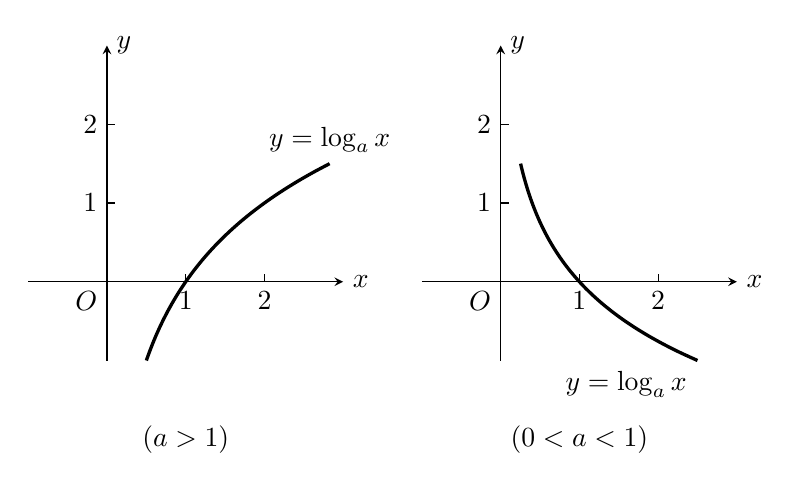
\begin{tikzpicture}[>=stealth]
\begin{scope}
    \draw[->](-1,0)--(3,0)node[right]{$x$};
    \draw[->](0,-1)--(0,3)node[right]{$y$};
\node [below left]{$O$};
\foreach \x in {1,2}
{
    \draw(\x,0)node[below]{$\x$}--(\x,.1);
    \draw(0,\x)node[left]{$\x$}--(.1,\x);
}
\node at (1,-2){$(a>1)$};
\draw[domain=-1:1.5, smooth, very thick]plot(2^\x, \x)node[above]{$y=\log_a x$};

\end{scope}
\begin{scope}[xshift=5cm]
\draw[->](-1,0)--(3,0)node[right]{$x$};
\draw[->](0,-1)--(0,3)node[right]{$y$};
\node [below left]{$O$};
\foreach \x in {1,2}
{
    \draw(\x,0)node[below]{$\x$}--(\x,.1);
    \draw(0,\x)node[left]{$\x$}--(.1,\x);
}
\node at (1,-2){$(0<a<1)$};
\draw[domain=1.5:-1, smooth, very thick]plot(0.4^\x, \x)node[below left]{$y=\log_a x$};

\end{scope}
\end{tikzpicture}
\end{center}

这里,类似于指数函数也应做几点说明(请读者自己考虑)。

\begin{example}
    在同一坐标系中,画出函数$y=\log_2 x$, $y=\log_3 x$, $y=\log_{\tfrac{1}{2}}x$, $y=\log_{\tfrac{1}{3}}x$的图象。
\end{example}

\begin{solution}
    利用描点法先画出$y=\log_2 x$与$y=\log_3 x$
的图象,再
利用关于$x$轴的对称性画出$y=\log_{\tfrac{1}{2}}x$与$y=\log_{\tfrac{1}{3}}x$
的图象。
\end{solution}

\begin{note}
    从图3.16可以看出,当底数
$a>1$时,$a$越大曲线越靠
近$x$轴与$y$轴,这同指数函数的情况是一致的(为什么?),
而当$0<a<1$时,结论恰恰相反。
\end{note}

\begin{figure}[htp]
    \centering
\begin{tikzpicture}[>=stealth]
\draw[->](-1,0)--(6,0)node[right]{$x$};
\draw[->](0,-3)--(0,3)node[left]{$y$};
\node [below left]{$O$};
\foreach \x in {1,2,3,4,5}
{
    \draw(\x,0)node[below]{$\x$}--(\x,.1);
}
\foreach \x in {-1,-2,1,2}
{
    \draw(0,\x)node[left]{$\x$}--(.1,\x);
}

\draw[domain=-1.5:1.6, smooth, thick]plot(3^\x,\x)node[below]{$y=\log_{3}x$};

\draw[domain=-1.75:2.4, smooth, very thick]plot(2^\x,\x)node[above]{$y=\log_{2}x$};

\draw[domain=-1.5:1.6, smooth, dashed, thick]plot(3^\x,-\x)node[above]{$y=\log_{\tfrac{1}{3}}x$};

\draw[domain=-1.75:2.4, smooth,  dashed,very thick]plot(2^\x,-\x)node[below]{$y=\log_{\tfrac{1}{2}}x$};

\foreach \x in {(2,1), (4,2)}
{
    \fill \x circle(2pt)node[above]{$\x$};
} 

\fill (3,1) circle(2pt)node[below]{$(3,1)$};
\foreach \x in {(2,-1), (4,-2)}
{
    \fill \x circle(2pt)node[above]{$\x$};
}
\fill (3,-1)circle(2pt)node[above right]{$(3,-1)$};
\fill(.5,1) circle(2pt)node[above right]{$\left(\tfrac{1}{2},1\right)$};
\fill(.5,-1) circle(2pt)node[below right]{$\left(\tfrac{1}{2},-1\right)$};


\end{tikzpicture}
    \caption{}
\end{figure}


\begin{example}
\begin{enumerate}[(1)]
    \item 若$\log_a 3>\log_b 3>0$,则$a$、$b$、1的大小顺序是\blank;
    \item 若$\log_a 0.3<\log_b 0.3<0$,则$a$、$b$、1的大小顺序是\blank。
\end{enumerate}
\end{example}

\begin{analyze}
    从图3.15可以直观地看出结论,也可以通过对条件式的变形解决问题。
\end{analyze}

\begin{solution}
\begin{enumerate}[(1)]
    \item 从图3.15可见,当$x\in (1,+\infty)$时,对于相同的$x$,若$y>0$(即$a>1$)时,必有$a$越大,$y$越小,从而知道$1<a<b$.
    
    若从$\log_a 3>\log_b 3>0$变形着手,有
\[\frac{1}{\log_3 a}>\frac{1}{\log_3 b}>0 \qquad \text{(化异底为同底)}\]

$\therefore\quad \log_3 b>\log_3 a>0\Longrightarrow \log_3 b>\log_3 a>\log_3 1$

利用$\log_3 x$是增函数,立刻有$b>a>1$.
\item 当$\log_a 0.3<\log_b 0.3<0$时,有
\[\frac{1}{\log_{0.3} a}<\frac{1}{\log_{0.3} b}<0\]

$\therefore\quad 0>\log_{0.3} a>\log_{0.3} b \Longrightarrow \log_{0.3} 1>\log_{0.3} a>\log_{0.3} b$

利用$\log_{0.3} x$是减函数,立刻有$1<a<b$.
\end{enumerate}
\end{solution}

\begin{example}
求下列函数的定义域:
\begin{multicols}{2}
\begin{enumerate}[(1)]
    \item $y=\log_{0.1}|x|$
    \item $y=\log_3 (4-x^2)$
    \item $y=\frac{1}{\log_3(3x+5)}$
    \item $y=\sqrt{\log_{0.1}(4x-3)}$
\end{enumerate}
\end{multicols}
\end{example}

\begin{solution}
\begin{enumerate}[(1)]
    \item $D=\{x\mid x\in\R,\; x\ne 0\}$
    \item $4-x^2>0,\; x\in(-2,2)$
    
$\therefore\quad D=(-2,2)$

\item 要使$y$有意义,须$\log_3(3x+5)\ne 0$,即$\begin{cases}
    3x+5\ne 1\\ 3x+5>0
\end{cases}$

$\therefore\quad 0<3x+5\ne 1\Longleftrightarrow -\frac{5}{3}<x\ne -\frac{4}{3}$

$\therefore\quad D=\left(-\frac{5}{3},-\frac{4}{3}\right)\cup\left(-\frac{4}{3},+\infty\right)$

\item 要使$y$有意义,须$\log_{0.1}(4x-3)\ge 0$,即$0<4x-3\le 1$,

解之,得
$\frac{3}{4}<x\le 1$

$\therefore\quad D=\left(\frac{3}{4}, 1\right]$
\end{enumerate}
\end{solution}

\begin{example}
    比较下列各题中两个数的大小。
    \begin{multicols}{2}
\begin{enumerate}[(1)]
    \item $\log_3 2.1$与$\log _3 2.8$
    \item $\log_{0.2}7.1$与$\log_{0.2}5.4$
    \item $\log_{a}4.4$与$\log_a 5.5$\quad $(0<a\neq1)$
    \item $(\lg a)^{8.1}$与$(\lg a)^{2.5}$\quad $(1<a\neq10)$
\end{enumerate}        
    \end{multicols}

\end{example}

\begin{solution}
\begin{enumerate}[(1)]
\item $\because \quad $对数函数$y=\log_3 x$单调递增,且$2.1<
2.8$, 

$\therefore\quad \log_3 2.1<\log_3 2.8$
\item $\because\quad $对数函数 $y=\log_{0.2}x$ 单调 递减,且$7.1>
5.4$

$\therefore\quad \log_{0.2}7.1<\log_{0.2}5.4$
\item 当$a>1$时,$y=\log_3 x$单调递增,且$4.4<5.5$,

$\therefore\quad \log_a 4.4< \log _{a}5.5$

当$0<a<1$时, $y=\log_a x$单调递减,且$4.4<5.5$,

$\therefore \quad \log_a 4.4> \log_a 5.5$
\item 当$a\in(1,10)$时,$0<\lg a<1$, 指数函数
$y=(\lg a)^{x}$单调递减,且$3.1>2.5$,

$\therefore\quad (\lg a)^{8.1}<(\lg a)^{2.5}$

当$a\in(10,+\infty)$时,$\lg a>1$, 指数函数
$y=(\lg a)^{x}$单调递增,且$3.1>2.5$,

$\therefore\quad (\lg a)^{8.1}>(\lg a)^{2.5}$
\end{enumerate}
\end{solution}

\begin{example}
 比较$\log_3 0.4$ 与$-\frac12$的大小.   
\end{example}

\begin{analyze}
    不同类的对象难以比较。根据“任一实数都能写
成对数形式”,先把$-\frac12$写成对数.
\end{analyze}

\begin{solution}
    \[- \frac 12= \log_3 3^{- \frac 12}= \log_{3}\frac {\sqrt {3}}3\]

$\because \quad y= \log_3 x$ 单调递增,且$0.4<\frac{\sqrt{3}}{3}.$

$\therefore \quad \log_3 0.4< \log_{3}\frac{\sqrt{3}}{3}$, 即$\log_3 0.4< - \frac 12.$    
\end{solution}

\begin{example}
    比较下列各题中两个数的大小
\begin{multicols}{2}
\begin{enumerate}[(1)]
    \item $\log_2 3$与$\log_7 6$
    \item $\log_{0.2}0.4$与$\log_2 0.7$
\end{enumerate}
\end{multicols}
\end{example}

\begin{analyze}
  因为两对数的底不同,故不能直接利用对数函数
的单调性比大小。若用换底公式做,也难以奏效。我们用
“中间值法”试一试。 常用的中间值是0或1.  
\end{analyze}

\begin{solution}
\begin{enumerate}[(1)]
    \item $\because\quad \log_2 3 >1$ ($\because\quad \log_2 3>\log_2 2=1$)
    
而$\log_7 6<1$ ($\because\quad \log_7 6<\log_7 7=1$)

$\therefore\quad \log_2 3 >\log_7 6$
\item $\because\quad \log_{0.2} 0.4 >0$ ($\because\quad \log_{0.2} 0.4>\log_{0.2} 1=0$)
    
而$\log_2 0.7<0$ ($\because\quad \log_2 0.7<\log_2 1=0$)

$\therefore\quad \log_{0.2} 0.4 >\log_2 0.7$
\end{enumerate}
\end{solution}

\begin{example}
    解不等式:
\begin{multicols}{2}
   \begin{enumerate}[(1)]
\item $\log_{0.1}(x^2-2x-2)>0$;
\item $\log_a(x^2-x)\ge \log_a (x+1)\quad (a>1)$
\end{enumerate} 
\end{multicols}

\end{example}

\begin{analyze}
    解不等式就是求未知数$x$的取值范围。就对数不等式而言,当然既要考虑对数函数的定义域,又要考虑对数函数的增减性。
\end{analyze}

\begin{solution}
\begin{enumerate}[(1)]
    \item 由于$\log_{0.1}1=0$,原不等式可改写成
\begin{equation}
    \log_{0.1}(x^2-2x-2)>\log_{0.1}1   \tag{1}
\end{equation}
由(1)
\begin{align}
    x^2-2x-2>0, \quad \text{(由定义域)} \tag{2}\\
    x^2-2x-2>0, \quad \text{(由增减性)} \tag{3}
\end{align}
解(2), 得 $x<1-\sqrt{3}$, 或$x>1+\sqrt{3}$

解(3), 得 $-1<x<3$

$\therefore\quad $原不等式的解集为$(-1,1-\sqrt{3})\cup (1+\sqrt{3},3)$.

\item 根据原不等式
\begin{align}
    x^2-x>0,&\quad \text{(由定义域)} \tag{4}\\
    x+1>0,&\tag{5}\\
    x^2-x\ge x+1,&\quad \text{(由增减性)} \tag{6}
\end{align}

由(5)、(6)可推得(4),所以(4)可省掉。

解(5),得$x>-1$;解(6),得$x\le 1-\sqrt{2}$,或$x\ge 1+\sqrt{2}$.

$\therefore\quad $原不等式的解集为
\[\left(-1,1-\sqrt{2}\right]\cup \left[1+\sqrt{2},+\infty\right)\]
\end{enumerate}
\end{solution}

\begin{note}
    解对数不等式的基本方法是转化为代数不等式组,这种转化既要考虑定义域,又要考虑增减性,否则前后可能不同解(不等价)。

    当式子中含参数时,要树立“讨论”的意识,如例4中的(3)、(4)。
\end{note}

\begin{example}
求证:$2<\frac{1}{\log_2 19}+\frac{2}{\log_3 19}+\frac{2}{\log_5 19}<3$
\end{example}

\begin{analyze}
    将三个不同底的对数化成同底。
\end{analyze}

\begin{proof}
\[\begin{split}
    \frac{1}{\log_2 19}+\frac{2}{\log_3 19}+\frac{2}{\log_5 19}&=\log_{19}2+2\log_{19}3+2\log_{19}5\\
    &=\log_{19}(2\times 3^2\times 5^2)=\log_{19}450
\end{split} \]
利用$\log_{19}x$是增函数,得
\[2=\log_{19}19^2<\log_{19}450<\log_{19}19^3=3\]

$\therefore\quad 2<\frac{1}{\log_2 19}+\frac{2}{\log_3 19}+\frac{2}{\log_5 19}<3$
\end{proof}

\begin{example}
求函数$y=\log_a(x^2-2x)$的单调区间。
\end{example}

\begin{analyze}
这个函数可看作是由$y=\log_a u\; (0<a\ne 1)$与$u=x^2-2x$复合而成的。由于$0<a<1$和$a>1$时$\log_a u$的增减性不同,因此应分情况进行讨论;另一方面又要考虑到函数$y=\log_a(x^2-2x)$的定义域为$(-\infty,0)\cup (2,+\infty)$.
\end{analyze}

\begin{solution}
\begin{enumerate}[(1)]
    \item 若$0<a<1$时,$\log_{a}u$为单调减函数,而函数$u=x^2-2x=(x-1)^2-1$在$(-\infty,1)$上单调减,在$(1,+\infty)$上单调增。故$(-\infty,0)$是函数$y=\log_{a}(x^{2}-2x)$的单调增区间,$(2,+\infty)$是函数的单调减区间。
    \item 若$a>1$时,则$(-\infty,0)$ 是函数$y=\log_a(x^2-2x)$的单调减区间,$(2,+\infty)$是函数的单调增区间。
\end{enumerate}
\end{solution}

\section*{习题四}
\begin{center}
    \bfseries A
\end{center}

\begin{enumerate}
    \item 证明:在同一坐标系中函数$y=\log_a x$与$y=\log_{\tfrac1a}x\; (0<a\neq1)$的图象关于$x$轴对称。
    \item 求下列函数的定义域:
\begin{multicols}{2}
\begin{enumerate}[(1)]
    \item $y=\log_5(1+x)$
    \item $y=\frac{1}{\ln x}$
    \item $y=\log_{0.1}\frac{1}{1-3x^2}$
    \item $y=\sqrt{\log_3 x}$
    \item $y=3\sqrt{\log_2 x}$
    \item $y=\sqrt{\log_{0.2}(3-2x)}$
    \item $y=\sqrt{\lg(2x^2-9x-4)}$
    \item $y=\frac{\sqrt{1-\frac{2}{3}|x|}}{\log_{0.1}(x+1)}$
\end{enumerate}
\end{multicols}

\item 若$\log_5 6\cdot \log_6 7\cdot \log_7 8\cdot \log_8 9\cdot \log_9 10=m$,那么$m$的值属于下列哪个区间:
\[(0,1),\qquad (1,2),\qquad (2,3),\qquad (3,4)\]
\item 比较下列各题中两个数的大小:
\begin{multicols}{2}
\begin{enumerate}[(1)]
    \item $\log_5 7.8$与$\log_5 9.2$
    \item $\log_{0.3}5$与$\log_{0.3}8$
    \item $\lg 0.75$与$\lg 0.85$
    \item $\ln108$与$\ln105$
    \item $\log_{0.2}0.7$与$\log_5 0.8$
    \item $\ln 4.9$与$\log_{\tfrac{1}{\sqrt{2}}}8.5$
    \item $\log_{\tfrac{3}{2}}\frac{3}{4}$与$\log_{\tfrac{1}{3}}\frac{2}{3}$
    \item $\log_a 3.14$与$\log_a \pi\; (0<a\ne 1)$
    \item $(\lg m)^{-3.1}$与$(\lg m)^{-2.4}$ 
    
    $(m>1)$
    \item $\log_{10}a$与$\log_a 10\quad (a>1)$
    \item $\log_a b$与$\log_{\tfrac{1}{a}}b\quad (0<a<1)$
\end{enumerate}
\end{multicols}
\item 填空:
\begin{enumerate}[(1)]
    \item $\log_{\tfrac{1}{2}}x<2$的解集是\blank.
    \item $\log_{\sqrt{2}}x<6$的解集是\blank.
    
    (提示:把右边的常数写成对数形式)
    \item 设$f(x)=\log_2 x$,则$[f(x)]^2>f(x^2)$的解集是\blank.
\end{enumerate}

\item 解下列不等式:
\begin{enumerate}[(1)]
    \item $\log_{0.2}(x^2+x-1)\ge 0$
    \item $\lg (x^2+21x)>2$
    \item $\log_{0.2}(x^2-3x-4)\ge \log_{0.2}(2x+10)$
\end{enumerate}
\end{enumerate}

\begin{center}
    \bfseries B
\end{center}

\begin{enumerate}\setcounter{enumi}{6}
    \item 设$\frac{1}{\log_{\tfrac{1}{2}}\frac{1}{3}}+\frac{1}{\log_{\tfrac{1}{5}}\frac{1}{3}}=n$,那么$n$属于下列哪个区间:
    \[(-2,-1),\quad (1,2),\quad (-3,-2),\quad (2,3)\]
\item 求证:
\begin{enumerate}[(1)]
\item $2< \frac 1{\log _{13}7}+ \frac 1{\log _{5}7}< 3$ ,

\item $4< \frac 3{\log _{2}e}+ \frac 2{\log _{3}e}< 5$ ,

\item $1< \frac 1{\log _{2}11}$ $+ \frac 1{\log _{3}11}$ $+ \frac 1{\log _{4}11}$ $+ \frac 1{\log _{5}11}< 2$.
\end{enumerate}
\item  若$\log_m(e-2)>\log_n(e-2)>0$, 试指出$m,n$与1的大
小顺序。
\item 解不等式:
$\log_{a}\left(2x^{2}-4x\right)\ge \log_{a}\left(x^{2}-4x+1\right)、\quad (0<a\neq1).$
\item 解下列不等式:
\begin{enumerate}[(1)]
    \item $\frac 1{\log _2x}- \frac 1{\log _2x- 1}< 1$
    \item $\log_{x}5- 2\log_{\sqrt {5}}x> 3\quad ( x> 1) $
    \item $\log_2\left(\frac23\right)^x+\log_2\left(\frac49\right)^{2x}<\log_2\left(\frac23\right)^5$
    \item $\log_2 x-\log_{\sqrt{x}}2<1 $
    \item $\log_{kx}x+\log_x (kx)^2>0\quad (0<k<1)$
    \item $\frac{1}{\log_{x-1}4}-\frac{1}{\log_{5-x}4}>0$
    \item $\log_{\tfrac{1}{2}}\left|\frac{1}{x-1}\right|>\log_{\tfrac{1}{2}}\left|\frac{2}{x+3}\right|+1$
\end{enumerate}

\item 求下列函数的单调减区间:
\begin{multicols}{2}
\begin{enumerate}[(1)]
    \item $y=\log_a (-x^2+6x-5)$
    \item $y=2^{|\lg x|}$
\end{enumerate}
\end{multicols}
\item 判断函数$f(x)=\lg\left(x+\sqrt{x^2+1}\right)$的奇偶性。
\end{enumerate}

\section{指数方程和对数方程}
在指数中含有未知数的方程叫做\textbf{指数方程}。

在对数记号中的真数或底数中含有未知数的方程叫做\textbf{对数方程}。

在这两类方程中,我们只能解一些特殊的方程。请看下面的例子。

\begin{example}
    解方程$4^x=2^{x+1}$.
\end{example}

\begin{solution}
    原方程可化为$$2^{2x}=2^{x+1}$$
根据指数函数
$y=2^u\; (u\in\R)$
的单调性,两个同底的幂相等,
当且仅当它们的幂指数相等,所以上面的方程同解于(或说
成“等价于”,记为$\Longleftrightarrow$)
\[2x=x+1\] 
$\therefore\quad x=1$.
\end{solution}

\begin{note}
    这里决定性的一步是把两个幂“化成同底”。
\end{note}

\begin{example}
     解方程$3^{x+1}+9^x-18=0$.
\end{example}

\begin{solution}
    原方程可化为
\[3\cdot 3^x +(3^x)^2-18=0\]
令$3^x=y$,这个方程就写成
\[y^2+3y-18=0\]
解之得:$y_1=3,\qquad y_2=-6$

由$3^x=3$,得$x=1$;
$3^x=-6$
不符合指数函数的性质,应
舍去。

$\therefore\quad $原方程的解是
$x=1$.
\end{solution}

\begin{note}
    这里使用换元法:
$y=3^x$,是解方程或不等式常
用的方法之一。
\end{note}

\begin{blk}
    方程
$2^{x+1}+3\cdot 2^{1-x}-8=0$
能用换元法解吗?
\end{blk}

\begin{example}
   某厂生产的彩电的台数,如果每年平均比上一年
增长10.4\%,约过多少年产量才能翻一番(结果保留一个有
效数字)? 
\end{example}

\begin{solution}
    设约过$x$年,产量可以翻一番,由题意可得
\[1\cdot (1+10.4\%)^x=2\]
即:$1.104^x=2$,两边取对数,得:
\[x\lg 1.104=\lg 2\]

$\therefore\quad x=\frac{\lg 2}{\lg 1.104}=\frac{0.3010}{0.0429}\approx 7$

答:约经过7年.
\end{solution}

以上三例讲的是\textbf{解指数方程的基本方法}:同底法(关键
是能化成
$a^{f(x)}=a^{g(x)}$
的形式,其中
$0<a\ne 1$);换元法(关
键是能看得出隐含了哪个“元”);取对数法。

\begin{example}
  解方程
  \begin{equation}
 \lg(x^2+11x+8)-\lg(x+1)=1\tag{1}     
  \end{equation}
\end{example}

\begin{solution}
    方程(1)等价于(同解于)
\[\begin{cases}
    x^2+11x+8>0,&\text{(由定义域)}\\
    x+1>0,&\text{(由定义域)}\\
    \lg\frac{x^2+11x+8}{x+1}=\lg10,&\text{(由单调性)}\\
\end{cases}\Longleftrightarrow \begin{cases}
    x^2+11x+8>0,&(2)\\
    x+1>0,&(3)\\
    \frac{x^2+11x+8}{x+1}=10,&(4)
\end{cases}\]
解(4),得:$x_1=-2,\quad x_2=1$

$x_1$不满足(3), 舍去;$x_2$满足(2)、(3)

$\therefore\quad x=1$是(1)的解.
\end{solution}

\begin{note}
    解对数方程时,首先应考虑定义域,从而转化为
代数不等式与方程的混合组。\textbf{解混合组的一般方法}是先求出
方程的解,再把它代入不等式。若都适合,它就是混合组的
解,否则,一定不是混合组的解。
\end{note}

\begin{example}
    解方程
    \begin{equation}
\log_2(5x^2-1)-1=\log_2 x+log_2 2x \tag{1}
    \end{equation}
\end{example}

\begin{solution}
\[\text{方程(1)}\Longleftrightarrow\begin{cases}
    x>0, \quad \text{(由定义域)}& (2)\\
    \log_2\frac{5x^2-1}{2}=\log_2(x\cdot 2x), &(3)
\end{cases}\]
\[(3)\Longleftrightarrow \begin{cases}
    5x^2-1>0\\
    x\ne 0\\
    \frac{5x^2-1}{2}=2x^2
\end{cases}\]
解之,得:$x_1=1,\quad x_2=-1$.

$x_1=1$适合(2);$x_2=-1$不适合(2),舍去。

$\therefore\quad x=1$是(1)的解。
\end{solution}


\begin{example}
    解方程
    \begin{equation}
        2log_{25}x+\log_x 25=3 \tag{1}
    \end{equation}
\end{example}

\begin{solution}
\begin{equation}
    (1)\Longleftrightarrow 2\log_{25}x+\frac{1}{\log_{25}x}=3 \tag{2}
\end{equation}
令$\log_{25}x=y$,则(2)变为
\[2y+\frac{1}{y}=3\Longleftrightarrow 2y^2-3y+1=0\; (y\ne 0)\]
解之,得:$y_1=1,\quad y_2=\frac{1}{2}$.

由$\log_{25}x=1$,得$x_1=25$;
由$\log_{25}x=\frac{1}{2}$,得$x_2=25^{\tfrac{1}{2}}=5$. $x_1,x_2$都适合(2)

$\therefore\quad $方程(1)的解集是$\{25,5\}$
\end{solution}


\begin{example}
    解方程
\begin{equation}
    \log_{2x^2-1}(3x^{2}-2x-1)=1 \tag{1}
\end{equation}
\end{example}

\begin{solution}
\[\text{方程(1)}\Longleftrightarrow \begin{cases}
    3x^{2}-2x-1>0,\quad \text{(由定义域)}& (2)\\
    0<2x^2-1\ne 1 & (3)\\
    3x^{2}-2x-1=2x^2-1 ,\quad \text{(由单调性)}& (4)
\end{cases}\]
解(4), 得 $x_1=0,\quad x_2=2$。

$x_1$不满足(2), 是增根,舍;$x_2$满足(2)、(3).

$\therefore \quad x= 2$是原方程的解。
\end{solution}

以上四例讲的是\textbf{解对数方程的基本方法}:转化成同解的
混合组,或者用换元法处理。

再研究几个例题。

\begin{example}
    解方程$x^{2\lg x}=10\cdot  x$
\end{example}

\begin{analyze}
    在幂$x^{2\lg x}$的底数与指数中都含有$x$, 但等号两边同取以10为底的对数(应该想到,两边都为正数,所以允许取对数),原方程就变成以$\lg x$为元的方程了。
\end{analyze}

\begin{solution}
    由于$x>0$, 方程两边皆正,取常用对数,得
$$2\lg x\cdot \lg x=1+lg x$$
令$\lg x= y$, 得$2y^2- y- 1= 0$。解之,得$y_1=1,\quad y_2=-\frac{1}{2}$.

由$\lg x=1$,得$x=10$;由$\lg x=-\frac{1}{2}$,得$x=\frac{\sqrt{10}}{10}$.

经检验,$x_1=10$,$x_2=\frac{\sqrt{10}}{10}$都是原方程的解。
\end{solution}

\begin{example}
    解不等式$x^{\log_a x}>\frac{x^{\tfrac{9}{2}}}{a^2}$
\end{example}

\begin{analyze}
    取以$a$为底的对数,就变成以$\log_a x$为元的不等式了。
\end{analyze}

\begin{solution}
由于$x>0$,不等式两边皆正,可以取以$a$为底的对数。
\begin{enumerate}
    \item 当$a>1$时,$\log_a u$是$u$的增函数,得:
    \[\log_a x\cdot \log_a x>\frac{9}{2}\log_a x-2\log_a a\]
令$\log_a x=y$,得:$2y^2-9y+4>0$,解之,得:$y<\frac{1}{2}$或$y>4$,即:
\[\log_a x<\frac{1}{2},\quad \text{或}\quad \log_a x>4\]

$\therefore\quad 0<x<\sqrt{a}$,或$x>a^4$.

\item 当$0<a<1$时,$\log_a u$是$u$的减函数,得
\[\log_a x\cdot \log_a x< \frac{9}{2}\log_a x-2\log_a a\]
令$\log_a x=y$,得:$2y^2-9y+4<0$,解之,得:$\frac{1}{2}<y<4$,即:
\[\frac{1}{2}<\log_a x<4\Longleftrightarrow \log_a a^{\tfrac{1}{2}}<\log_a x<\log_a a^4\]

$\therefore\quad \sqrt{a}>x>a^4$
\end{enumerate}
\end{solution}

\begin{note}
    解题中,当需要对不等式两边取以$a$为底的对数
时,要特别注意参数$a$的不同取值对对数函数增减性的影响,
通过此例应很好地理解这一点。
\end{note}



\begin{example}
解方程:
\begin{multicols}{2}
\begin{enumerate}[(1)]
    \item $x+\lg x=3$
    \item $2^x=\log_3(x+3)$
\end{enumerate}
\end{multicols}
\end{example}

\begin{analyze}
    这两个方程都是我们未曾见过的类型。无现成模
式可用。此时,“转化”的思想有可能使我们找到解决问题的
途径。

对于(1)原方程改写作
\begin{equation}
    \lg x=3-x\tag{1}
\end{equation}
令$f(x)=\lg x$,$g(x)=3-x$
。以函数的观点来看,方程(1)的解
就是使$f(x)$与$g(x)$
的函数值相等的$x$值。而这两个函数都是
我们所熟知的,从而,可用图象法解决问题。
\end{analyze}

\begin{figure}[htp]
    \centering
\begin{minipage}{.45\textwidth}
    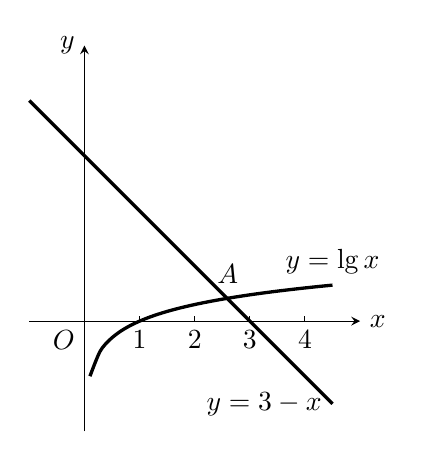
\begin{tikzpicture}[>=stealth, scale=.7]
\draw[->](-1,0)--(5,0)node[right]{$x$};
\draw[->](0,-2)--(0,5)node[left]{$y$};
\node[below left]{$O$};
\draw[domain=-1:4.5, very thick]plot(\x, 3-\x)node[left]{$y=3-x$};
\draw[domain=.1:4.5, very thick, smooth]plot(\x,{log10(\x)})node[above]{$y=\lg x$};
\foreach \x in {1,2,3,4}
{
    \draw(\x,0)node[below]{\x}--(\x,.1);
}        
\node at (2.6,.5)[above]{$A$};
\end{tikzpicture}
 \caption{}    
\end{minipage}\hfill
   \begin{minipage}{.45\textwidth}
    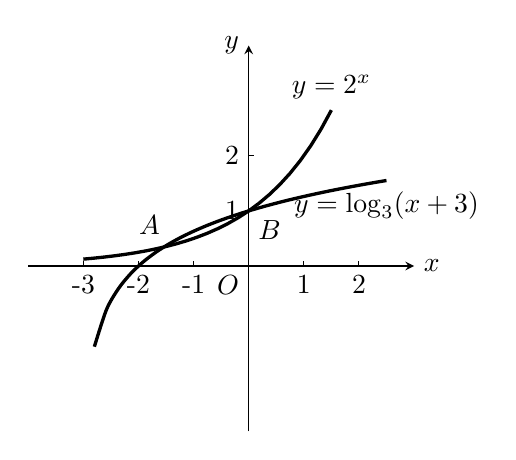
\begin{tikzpicture}[>=stealth, scale=.7]
    \draw[->](-4,0)--(3,0)node[right]{$x$};
\draw[->](0,-3)--(0,4)node[left]{$y$};
\node[below left]{$O$};        

\draw[domain=-3:1.5, very thick]plot(\x, 2^\x)node[above]{$y=2^x$};
\draw[domain=-2.8:2.5, very thick, smooth]plot(\x,{log2(\x+3)/log2(3)})node[below]{$y=\log_3(x+3)$};
\foreach \x in {1,-2,-3,-1,2}
{
    \draw(\x,0)node[below]{\x}--(\x,.1);
}    
\foreach \x in {1,2}
{
    \draw(0,\x)node[left]{\x}--(.1,\x);
}   
\node at (0,1)[below right]{$B$};
\node at (-1.8,.4)[above]{$A$};
\end{tikzpicture}
 \caption{}    
\end{minipage}
\end{figure}




\begin{solution}
\begin{enumerate}[(1)]
    \item 在同一坐标系中分别作出$f(x) = \lg x$与$g(x)=3-x$的图象(图3.17). 两图象相交于$A$ 点(此时,两个函数值相等),$A$的横坐标$x\approx2.6$. 这个值近 似地使$f(x)=g(x)$. 所以,$x=2.6$ 是方程(1)的近 似解,也就是原方程的近似解。(应该看 到,对于(1)我们是无法 求出它的准确解的,想想这是为什么?)
    \item 类似于(1), 用图象法。在同一坐标系中分别作出函数$f(x)=2^{x}$与$g(x)=\log_{3}(x+3)$的图象(图3.18)。两图象相交于$A,B$两点。从图上可以看出点$A$的横坐标$x_1\approx-1.8$, 点$B$的横坐标$x_2=0$. 所以$x_1=-1.8$是方程(2)的近似解,$x_2=0$是(2)的解。
\end{enumerate}
\end{solution}

\begin{note}
此例使我们又一次看到:方程、不等式、函数之
间的密切关系。一般说来,运用函数的观点去透视方程和不
等式的问题常常有助于问题的解决。
\end{note}    

\begin{example}
方程$\lg(ax)\lg(ax^2)=4$的所有的解都大于1,求实数$a$的范围。
\end{example}

\begin{solution}
$\because\quad ax^2>0,\; ax>0$, \qquad $\therefore\quad a>0,\; x>0$.

原方程可写成
\begin{equation}
   2\lg^2 x+3\lg a\cdot \lg x+\lg^2 a-4=0 \tag{1} 
\end{equation}

$\because\quad $方程所有的解都大于1,

$\therefore\quad $以$\lg x$为元的方程(1)的所有的解都大于0。于是:
\[\begin{cases}
\Delta =(3\lg a)^2-4\cdot 2(\lg^2 a-4)\ge 0\\
\frac{-3\lg a}{2\cdot 2}>0\\
\frac{\lg^a-4}{2}>0
\end{cases}\Longrightarrow \begin{cases}
    \lg^2 a+32>0\\
    \lg a<0\\
    |\lg a|>2
\end{cases}\]
$\therefore\quad \lg a<-2$,
即:$0<a<\frac{1}{100}$.
\end{solution}

\section*{习题五}
\begin{center}
    \bfseries A
\end{center}

\begin{enumerate}
    \item 解下列指数方程(口答):
\begin{multicols}{2}
\begin{enumerate}[(1)]
    \item $3^{\tfrac{1}{x}}=9$
    \item $\left(\frac{1}{4}\right)^{-x}=64$
    \item $5^{(x-1)(x+2)}=1$
    \item $2^x=100$
    \item $\left(\frac{3}{7}\right)^{3x-7}=\left(\frac{7}{3}\right)^{2x-8}$
    \item $3^x=5^x$
\end{enumerate}
\end{multicols}

\item 解下列指数方程:
\begin{multicols}{2}
\begin{enumerate}[(1)]
    \item $6^{2x+4}=2^{x+8}\cdot 3^{3x}$
    \item $3^{x^2+1}+3^{x^2-1}=270$
    \item $4^{x+1}+\frac{64}{4^x}=40$
    \item $7\cdot (3^{x+1})-5^{x+2}=3^{x+4}-5^{x+3}$
    \item $2^{2x+1}-33.2^{x-1}+4=0$
    \item $3^{x+2}+3^{-x}-6=0$
    \item $2^{x+1}+3\cdot 2^{1-x}-8=0$
    \item $25^x +35^x=49^x$
    \item $2^{2x}+3^{3x}=9\cdot 2^{x+3}$
\end{enumerate}
\end{multicols}

\item 解下列对数方程:
\begin{multicols}{2}
\begin{enumerate}[(1)]
    \item $\lg(x^2-x-3)=\lg(2x+1)$
    \item $\lg x+\lg(x+3)=1$
    \item $\log_2 (9x^2-20)-2=\log_2 6+\log_2 x$
    \item $2(\log_3 x)^2+\log_3 x-1=0$
    \item $\log_3 \log_4\log_5 x=0$
    \item $2\log_x 25-3\log_{25}x=1$
    \item $\log_{16}x+\log_4 x+\log_2 x=7$
\end{enumerate}
\end{multicols}
\end{enumerate}

\begin{center}
    \bfseries B
\end{center}
\begin{enumerate}\setcounter{enumi}{3}
    \item 解下列方程:
\begin{enumerate}[(1)]
    \item $\left(\sqrt{3+2\sqrt{2}}\right)^x+\left(\sqrt{3-2\sqrt{2}}\right)^x=6$
\begin{multicols}{2}
    \item $2\log_x 3\cdot \log_{3x} 3=\log_{9\sqrt{x}}3$
    \item $\frac{1}{5-\log x}+\frac{2}{1+\lg x}=1$
    \item $3^{2-\log_3 x}=81x$
    \item $x^{\lg x}=5\cdot 2^{\lg x^2-1}$
    \item $x^{\lg x+2}=1000$    
\end{multicols}
\end{enumerate}

\item 解不等式:$|x-2|^{\log_{4}(x+2)-\log_{2}x}<1$
\item 解不等式:$\log_{4}5-2\log_{\sqrt{5}}x>3$

\item 解方程$\log_{4}(3x+10)\cdot\log_x 2=1$
\item 解方程$\log_{4}(2-x)=\log_{2}(x-1)-1$
\item 解方程$\log_{2}(2^{-x}-1)\cdot\log_{\tfrac{1}{1}}(2^{-x+1}-2)=-2$

\item 已知:$2\lg ( x- 2y) = \lg x+ \lg y$, 求$\frac xy$.

\item 求下列方程的解或近似解(精确到0.1)。
\begin{multicols}{2}
\begin{enumerate}[(1)]
    \item $3^{x}=4-x$
    \item $\lg x+x^{2}=0$
    \item $2^{x }- 1= \sqrt {x}$
    \item $|\log_3 x|- 3^{-x}= 0$
\end{enumerate}
\end{multicols}

\end{enumerate}

\begin{center}
    \bfseries C
\end{center}
\begin{enumerate}\setcounter{enumi}{11}
    \item 解方程 $3^x+4^x=5^x$.
\item 若$\lg 2x\cdot\lg3x=-a^2$有相异两实数解,求
\begin{enumerate}[(1)]
    \item 实数$a$的取值范围;
    \item 两实数解的乘积。
\end{enumerate}
\end{enumerate}

\section{本章小结}

\subsection{知识结构分析}

\subsubsection{幂函数的定义、图象和性质}

\begin{enumerate}
    \item 定义:函数$y=x^a\; (a\in \R$)叫做幂函数。中学阶段
只研究$a\in \Q$的情况,记作$y= x^n\; ( n \in \Q)$.
\item 由于$n\in \Q$, $n$可表示为$\frac qp$, 其中$p\in\mathbb{N}$, $q\in \Z$, 且
$|q|$、$p$互质。为便于研究,可分为$n>0$ 和 $n<0$ 两类情况。不妨设$p, q\in\mathbb{N}$, 且$p$、$q$互质,则$x^{n}$的意义分别为$\sqrt[p]{x^{q}}$和
$\frac{1}{\sqrt[p]{x^q}}$. 由此便可得出幂函数的基本性质(详见课文)。
\end{enumerate}

\subsubsection{指数函数和对数函数}

函数$y= a^x\quad ( a> 0,\;  a\neq1) $叫指数 函数,函数$y=\log_{a}x\quad (a>0,\; a\neq1)$叫对数函数。它们互为反函数,其图象关于直线$y=x$成轴对称图形.

\subsubsection{对数概念}
对数的运算法则、换底公式及对数恒等式(详见课文).

\subsubsection{指数方程和对数方程}
指数函数与对数函数都是一一映射,这是解指数方程与对数方程的主要依据,并由此转化为代数方程,解对数方程时应注意验根。

\subsection{几点说明}
\begin{enumerate}

\item 上一章学了函数概论——研究函数的基本思想和方法。本章就是运用这些思想研究了几类重要的初等函数——幂函数、指数函数和对数函数.

\item \textbf{数形结合}是研究函数的重要数学思想之一,要做到“依性作图,依图识性”。
\begin{enumerate}[(1)]
    \item 幂函数的性质可结合图3.19来掌握与记忆:
\begin{figure}[htp]
    \centering
\begin{tikzpicture}[>=stealth, scale=1.5]
\draw[->](-.5,0)--(3,0)node[below]{$x$};
\draw[->](0,-.5)--(0,3)node[left]{$y$};
\draw[dashed](1,0)node[below]{1}--(1,1)--(0,1)node[left]{1};
\draw[domain=0:2.5]plot(\x, \x)node[right]{$y=x$};
\draw[domain=0:1.65, smooth, dashed]plot(\x, \x^2)node[right]{$y=x^2$};
\draw[domain=0:1.4, smooth, dashed, very thick]plot(\x, \x^3)node[above]{$y=x^3$};
\draw[domain=0:2.5, smooth,  samples=1000,thick]plot(\x, {\x^(0.5)})node[above right]{$y=x^{\tfrac{1}{2}}$};
\draw[domain=0:2.5, smooth, samples=1000, very thick]plot(\x, {\x^(1/3)})node[right]{$y=x^{\tfrac13}$};
\draw[domain=0.35:2.5, smooth, ultra thick]plot(\x, 1/\x)node[right]{$y=x^{-1}$};
\draw[domain=0.58:2.5, smooth]plot(\x, {\x^(-2)})node[right]{$y=x^{-2}$};

\node[below left]{$O$};
\end{tikzpicture}
    \caption{}
\end{figure}


    例如,幂函数在第一象限内的图象均过点$(1,1)$,并在该点交汇;在区间$(1,+\infty)$上,$n$值越小,图象越靠近$x$轴,等等。

\item 指数函数和对数函数的性质可分别结合图3.20和图3.21,来理解与记忆:
\begin{figure}[htp]
    \centering
\begin{minipage}{.45\textwidth}
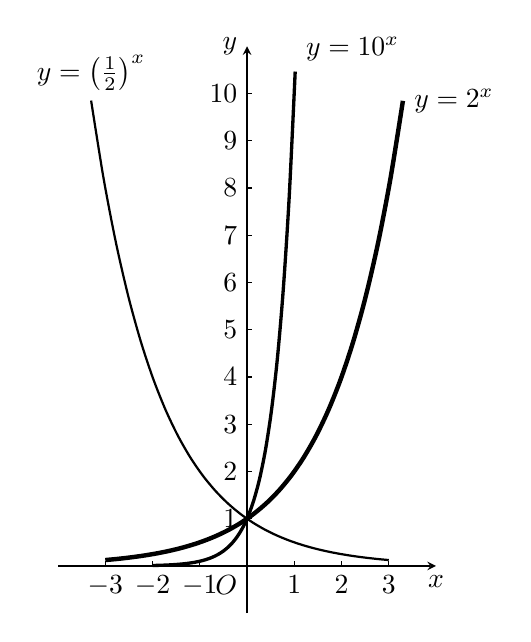
\begin{tikzpicture}[>=stealth, scale=.6]
\draw[->](-4,0)--(4,0)node[below]{$x$};
\draw[->](0,-1)--(0,11)node[left]{$y$};
\foreach \x in {1,2,...,10}
{
    \draw(0,\x)node[left]{$\x$}--(.1,\x);
}
\foreach \x in {1,2,3,-1,-2,-3}
{
    \draw(\x,0)node[below]{$\x$}--(\x,.1);
}
\draw[domain=3:-3.3, smooth, thick]plot(\x, 0.5^\x)node[above]{$y=\left(\frac{1}{2}\right)^x$};
\draw[domain=-2:1.02, smooth, very thick]plot(\x, 10^\x)node[above right]{$y=10^x$};
\draw[domain=-3:3.3, smooth, ultra thick]plot(\x, 2^\x)node[right]{$y=2^x$};
\node[below left]{$O$};
\end{tikzpicture}    
\caption{}
\end{minipage}   \hfill 
\begin{minipage}{.45\textwidth}
\begin{tikzpicture}[>=stealth, scale=.8]
    \node[below left]{$O$};
\draw[->](-1,0)--(6,0)node[below]{$x$};
\draw[->](0,-3)--(0,3)node[left]{$y$};
\draw[domain=.25:5, smooth, ultra thick]plot(\x, {log2(\x)})node[right]{$y=\log_2 x$};
\draw[domain=.25:5, smooth, very thick]plot(\x, {log2(\x)/log2(3)})node[right]{$y=\log_3 x$};
\draw[domain=.25:5, smooth, thick]plot(\x, -{log2(\x)})node[right]{$y=\log_{\tfrac{1}{2}} x$};
\foreach \x in {-2,-1,1,2}
{
    \draw(0,\x)node[left]{$\x$}--(.1,\x);
}
\foreach \x in {1,2,3,4,5}
{
    \draw(\x,0)node[below]{$\x$}--(\x,.1);
}
\end{tikzpicture}    
\caption{}
\end{minipage}   
\end{figure}


例如,指数函数的图象均在$x$轴上方,并且均过点$(0,1)$;指数函数$y=a^x$与$y=\left(\frac{1}{a}\right)^x$图象关于$y$轴对称。对于函数$y=a^x\; (a>1)$,在$(0,+\infty)$上$a$越大图象越接近$y$轴,在$(-\infty,0)$上$a$越大,图象越接近$x$轴。

对数函数图象均在$y$轴右侧,且均过点$(1,0)$;$y=\log_a x$与$y=\log_{\tfrac{1}{a}}x$图象关于$x$轴对称。对于$y=\log_a x$,在区间$(1,+\infty)$上,$a>1$时图象在$x$轴上方,且$a$越大越接近$x$轴;$0<a<1$时,图象在$x$轴下方,且$a$越小图象越接近$x$轴,等等。
\end{enumerate}
  \item \textbf{转化(化归)思想}在解指数方程和对数方程时得到了充分的体现。根据指数函数和对数函数是一一映射,从而转化为已经学习过的代数方程。转化时要注意转化的条件。对数方程转化为代数方程的条件是真数大于0,底数是大于0而不等于1的数。
\item \textbf{换元法}是解指数方程与对数方程的重要方法之一。一些较为复杂的方程,通过换元,有可能转化为较简单的指数方程和对数方程,从而可求其解。

例如$\log_2^2 x-3\log_2x-4=0$, $a^{2x}-5a^x+4=0$,等等。
\item  研究简单复合函数的某些性质的基本方法是:先将复合函数“\textbf{分解}”为若干个简单函数,然后把每个简单函数的基本性质“\textbf{综合}”起来考虑,便可得出复合函数的性质。

例如,确定函数$y=\left(\frac{1}{2}\right)^{x^2-3x}$的单调区间,其解法是:

设$y=\left(\frac{1}{2}\right)^t$, $t=x^2-3x=\left(x-\frac{3}{2}\right)^2-\frac{9}{4}$

$\because\quad x<\frac{3}{2}$时,$t(x)$是单调减函数,从而此时,$y=\left(\frac{1}{2}\right)^t$
为单调增函数;

同理可得$x>\frac{3}{2}$时,$y=\left(\frac{1}{2}\right)^t$为单调减函数。

从而得出$\left(-\infty, \frac{3}{2}\right)$是$y=\left(\frac{1}{2}\right)^{x^2-3x}$的单调增区间。$\left(\frac{3}{2},+\infty\right)$是$y=\left(\frac{1}{2}\right)^{x^2-3x}$的单调减区间。
\end{enumerate}

\section*{复习题三}
\begin{center}
\bfseries A    
\end{center}

一、选择题(有且只有一个正确答案):
\begin{enumerate}
    \item 若函数$y=(m^2-3m-17)x^{4m-m^2}$是幂函数,且其图象不经过坐标原点,则$m$的取值为\hfill (\qquad )
\begin{enumerate}[(A)]
    \item $m<0$或$m>4$
    \item $m<0$,或$m>4$,且$m\ne \frac{-3\pm\sqrt{77}}{2}$
    \item $m=-6$
    \item $m=3$
\end{enumerate}

\item 设$x=0.3^{-0.4}$, $y=\log_{0.3}0.4$, $z=\log_4 0.3$,则$x,y,z$间的大小顺序为\hfill (\qquad )
\begin{multicols}{4}
\begin{enumerate}[(A)]
    \item $z<y<x$
    \item $z<x<y$
    \item $x<z<y$
    \item $y<z<x$
\end{enumerate}
\end{multicols}

\item 函数$y=\log_{\tfrac{1}{2}}(2x-x^2)$的单调增区间为\hfill (\qquad )
\begin{multicols}{4}
\begin{enumerate}[(A)]
    \item $(1,+\infty)$
    \item $(-\infty,1)$
    \item $(0,1)$
    \item $(1,2)$
\end{enumerate}
\end{multicols}

\item 函数$y=\sqrt{\log_{\tfrac{1}{2}}(4x-3)}$的定义域为\hfill (\qquad )
\begin{multicols}{4}
\begin{enumerate}[(A)]
    \item $\left[\frac{3}{4},+\infty\right)$
    \item $\left(\frac{3}{4},1\right]$
    \item $(-\infty,1]$
    \item $\left[\frac{3}{4},1 \right]$
\end{enumerate}
\end{multicols}

\item 下列各函数中,既是偶函数,又在区间$(\infty,0)$上单调递减的是\hfill (\qquad )
\begin{multicols}{4}
\begin{enumerate}[(A)]
    \item $y=-x^{-2}$
    \item $y=-x^{\tfrac{2}{3}}$
    \item $y=-x^{\tfrac{1}{3}}$
    \item $y=x^{-2}$
\end{enumerate}
\end{multicols}
\end{enumerate}

二、填空题:
\begin{enumerate}
    \item 函数$y=1+\log_2 (x-2)$的反函数是\blank 
    \item 函数$y=\frac{\sqrt{x+2}}{\sqrt{\left(\frac{1}{5}\right)^x-1}}$的定义域是\blank
    \item 已知$y=\left(\frac{2}{\sqrt{5}}\right)^x$,当$x$\blank 时,$y>1$;当$x$\blank 时,$y=1$;当$x$\blank 时,$y<1$.
    \item 函数$y=3^x$与$y=-3^x$的图象关于\blank 对称;$y=4^x$与$y=4^{-x}$的图象关于\blank 对称;$y=3^x$与$y=-3^{-x}$的图象关于\blank 对称.
    \item $y=2^{x^2-2x-3},\quad x\in [-2,2]$,$y$的最小值是\blank; 最大值是\blank.
\end{enumerate}

三、解答题:
\begin{enumerate}
    \item 设$f(x)=\frac{1+x^2}{1-x^2}$,求证:
\begin{multicols}{2}
\begin{enumerate}[(1)]
    \item $f(x)$为偶函数
    \item $f\left(\frac{1}{x}\right)=-f(x)$
\end{enumerate}
\end{multicols}

\item 设$f(x)=\frac{e^x-e^{-x}}{2}$, $g(x)=\frac{e^x+e^{-x}}{2}$,求证:
\begin{enumerate}[(1)]
    \item $[g(x)]^2-[f(x)]^2=1$
    \item $f(2x)=2f(x)\cdot g(x)$
    \item $g(2x)=[f(x)]^2+[g(x)]^2$
\end{enumerate}

\item 在公共的定义域内,求证:
\begin{enumerate}[(1)]
\item 奇函数与奇函数的和仍为奇函数,偶函数与偶函数的和仍是偶函数;
\item 奇函数与奇函数的积是偶函数;
\item 奇函数与偶函数的积是奇函数;
\item 偶函数与偶函数的积是偶函数。
\end{enumerate}

\item 解下列方程:
\begin{multicols}{2}
\begin{enumerate}[(1)]
    \item $5^x+5^{x-1}=750$
    \item $4^x-2\times 6^x+9^x=0$
    \item $\log_7(\log_3 x)=-1$
    \item $\log_x x^x=2$
    \item $\lg(x-1)+\lg(x-2)=\lg(x+2)$
    \item $x^{2\lg x}=10x$
\end{enumerate}
\end{multicols}
\end{enumerate}

\begin{center}
    \bfseries B
\end{center}

\begin{enumerate}\setcounter{enumi}{4}
    \item 求下列函数的定义域、值域:
\begin{multicols}{2}
\begin{enumerate}[(1)]
    \item $y=\frac{x+1}{x+2}$
    \item $y=-\sqrt{x^2+25}$
    \item $y=\frac{1}{(x-1)(2x-1)}$
    \item $y=x+\sqrt{1-2x}$
\end{enumerate}
\end{multicols}

\item 求下列函数的定义域:
\begin{enumerate}[(1)]
    \item $y=\sqrt{3^x-9}$
    \item $y=\sqrt{1-a^x}\quad (0<a<1)$
    \item $y=\log_a(6x^2-x-2)\quad (a>0,\;\text{且}a\ne 1)$
    \item $y=\log_a(-x^2+4x-3)\quad (a>0,\;\text{且}a\ne 1)$
\end{enumerate}

\item \begin{enumerate}[(1)]
    \item 方程$3^{2x^2}=3^{5x+7}$与方程$2x^2=5x+7$的解集是否相等,为什么?
    \item 方程$\log_2 2x^2=\log_2 (x+6)$与方程$2x^2=x+6$的解集是否相等,为什么?
    \item 方程$\lg(x-1)+\lg(x-2)=\lg(x+2)$与方程$(x-1)(x-2)=x+2$的解集是否相等,为什么?
\end{enumerate}

\item 解下列方程组:
\begin{multicols}{2}
\begin{enumerate}[(1)]
    \item $\begin{cases}
        9^{x+y}=729\\ 3^{x-y-1}=1
    \end{cases}$
\item $\begin{cases}
    2^x\cdot 3^y=648\\
    3^x\cdot 2^y=432
\end{cases}$
\item $\begin{cases}
    \lg x+\lg y=5\\ \lg x-\lg y=3
\end{cases}$
\item $\begin{cases}
    x-y=90\\ \lg x+\lg y=3
\end{cases}$
  \end{enumerate}  
\end{multicols}

\end{enumerate}
